
In this Chapter we implement a finite element method (FEM) for an unstructured triangular mesh on a general polygonal domain in the plane.  Our code solves certain linear and nonlinear Poisson equation problems with reasonably-general boundary conditions.

The approach is to
\begin{center}
\emph{first do element-wise assembly of the residual equations,}
\end{center}
and thereby get a functioning \pSNES-based code.  No explicit matrix construction is needed in writing the initial code.  Only after making sure it works do we
\begin{center}
\emph{write additional code to assemble an approximate Jacobian matrix.}
\end{center}

We do the following new tasks in this Chapter:
\begin{itemize}
\item implement Neumann boundary conditions,
\item read a triangular mesh from a file into \PETSc \pVecs and \pISs,
\item index that mesh in an unstructured way, and
\item pre-allocate a \PETSc \pMat.
\end{itemize}

Similarly to the example in the last Chapter, the nonlinear system $\bF(\bu)=0$ seen by the \pSNES solver is the discretized weak form of the PDE.  Our construction of these equations roughly follows the implementations of Chapters \ref{chap:nl}--\ref{chap:of}, but without the structured grid and \pDMDA object.

The FEM ``stiffness'' matrix $A$, a major piece in typical FEM introductions \citep{Braess2007,Elmanetal2005}, arises here as the Jacobian when solving $\bF(\bu)=0$.  In our initial runs the \pSNES solver approximates this linear system through finite-differencing of evaluations of $\bF$.  Eventually we do assemble a Jacobian, but one that is only correct for the linear case.  For the smooth nonlinear case tested here, however, this ``Picard'' approximate linearization does a good job.

The example here contrasts with the rectangular-element ($Q^1$) FEM of the last Chapter by not using a \pDMDA-based structured grid.  Instead we implement our own ``naive'' mesh-topology infrastructure, which substantially increases our workload.  First, ASCII files generated by the \Triangle program define our input meshes.  Then a \PETSc \pIS ``index set'' type holds the global indices of nodes and triangles (elements).

In contrast with both earlier and later Chapters, our code only works on one MPI process.  However, at the end of the Chapter we briefly consider the additional constructs needed to distribute a mesh across many processes.  These considerations motivate the \pDMPlex example in Chapter \ref{chap:dp}.  The benefits of \PETSc's mesh-topology \pDM tools, including \pDMDA and \pDMPlex, become quite clear by forgoing them here.


\section{A 2D nonlinear Poisson problem}

\begin{marginfigure}
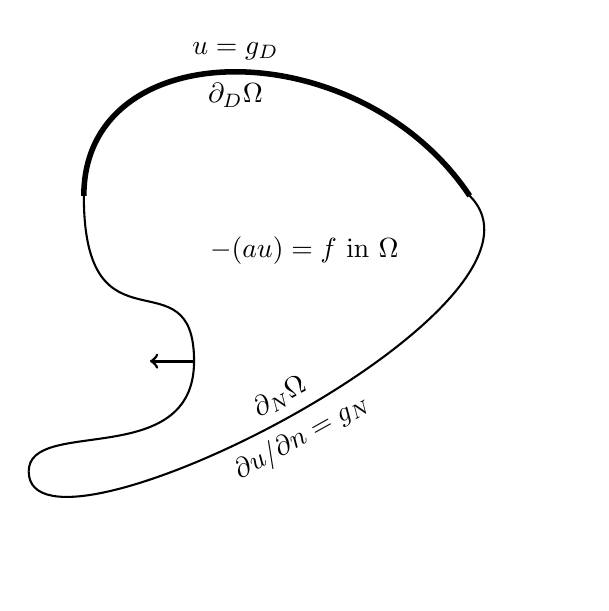
\begin{tikzpicture}[scale=0.7]
%\draw[gray,very thin] (-2,-6) grid (8,3);
\draw[line width=2pt] (0,0) .. controls (0,3) and (5,3) .. node[sloped,above] {$u=g_D$} node[sloped,below] {$\partial_D\Omega$} (7,0);
\draw[line width=0.75pt] (7,0) .. controls (9,-2) and (-1,-7) .. node[sloped,above] {$\partial_N\Omega$} node[sloped,below] {$\partial u/\partial n = g_N$} (-1,-5);
\draw[line width=0.75pt] (-1,-5) .. controls (-1,-4) and (2,-5) .. (2,-3);
\draw[line width=0.75pt] (2,-3) .. controls (2,-1) and (0,-3) .. (0,0);
\draw[->,line width=1.0pt] (2,-3) -- (1.2,-3) node[below] {$\bn$}; % normal vector
\draw (4,-1) node {$- \Div (a \grad u) = f$ in $\Omega$};
\end{tikzpicture}


\caption{Problem \eqref{eq:un:poissonstrong} on a domain.}
\label{fig:un:generalpoissondomain}
\end{marginfigure}

Let $\Omega \subset \RR^2$ be a bounded (open) region as in Figure \ref{fig:un:generalpoissondomain}.  We suppose its boundary $\partial\Omega$ is well-behaved, for example polygonal or Lipschitz-continuous \citep[section 1.2]{Ciarlet2002}.  Also we decompose the boundary into (measurable) disjoint subsets $\partial_D \Omega$ and $\partial_N \Omega$.

Chapter \ref{chap:st} solves the Poisson equation $- \grad^2 u = f$.  Here we allow a more general nonlinear form.  Let $a(u,x,y)$ and $f(u,x,y)$ be given and assume there is $\eps$ so that
\begin{equation}
a(u,x,y) \ge \eps > 0, \label{eq:un:uniformelliptic}
\end{equation}
that is, \emph{uniform ellipticity} \citep{Evans2010}.  Boundary conditions are also needed, and we allow nonhomogeneous Dirichlet and Neumann type.  Let $\partial u/\partial n = \bn \cdot \grad u$ where $\bn$ is the outward unit normal on $\partial \Omega$ (Figure \ref{fig:un:generalpoissondomain}).  The nonlinear Poisson \emph{strong form} we solve finds $u(x,y)$ so that
\begin{align}
- \Div \left(a(u,x,y) \grad u\right) &= f(u,x,y) \quad \text{ on } \Omega, \label{eq:un:poissonstrong} \\
u &= g_D \quad \text{ on } \partial_D \Omega, \notag \\
\frac{\partial u}{\partial n} &= g_N \quad \text{ on } \partial_N \Omega. \notag
\end{align}

The data of problem \eqref{eq:un:poissonstrong} includes a \emph{diffusion coefficient} $a$, a \emph{source term} $f$, \emph{Dirichlet data} $g_D$, and \emph{Neumann data} $g_N$.  For the purpose of numerical solutions we will assume these data are continuous.  Poisson problem \eqref{poissonsquare} in Chapter \ref{chap:st} is the homogeneous Dirichlet case where $\Omega$ is a square, $a = 1$, $f=f(x,y)$, $\partial_D \Omega = \partial \Omega$, $\partial_N \Omega = \emptyset$, and $g_D=0$.

More general boundary conditions are conceivable in \eqref{eq:un:poissonstrong}, in particular \emph{Robin} conditions $\alpha u + \beta \frac{\partial u}{\partial n} = \gamma$ where $\alpha,\beta,\gamma$ could vary along the boundary \citep{Elmanetal2005}; see Exercise \ref{chap:un}.\ref{exer:un:robin}.  One could also allow $a$ and/or $f$ to depend on the gradient of $u$; recall $a=|\grad u|^{p-2}$ in the $p$-Laplacian equation of Chapter \ref{chap:of}, for example, but our code is limited to problem \eqref{eq:un:poissonstrong}.

As \eqref{eq:un:poissonstrong} is stated there may be no solution where ``$\Div(a\grad u)$'' makes sense as a continuous function, even for polygonal regions and continuous data.  That is, there may be no $u\in C^2(\Omega) \cap C(\overline \Omega)$ so that \eqref{eq:un:poissonstrong} applies at all points.  On the other hand, at least in the linear case, a solution exists if we convert \eqref{eq:un:poissonstrong} to a weak formulation.  It already arose in Chapter \ref{chap:of} as the gradient of an objective function, but the weak form in this Chapter generally does not have a minimization origin; see Exercise \ref{chap:un}.\ref{exer:un:notminimization}.  Here we derive the weak form from the strong form simply by multiplying by a test function and integrating.


\section{Weak form with general boundary values}

Recall $L^2(\Omega)$ is the space of square-integrable real functions on $\Omega$ and that $W^{1,2}(\Omega)$ is the Sobolev space in which the gradient is also square integrable.\sidenote{See definition \eqref{eq:of:sobolevdefn}.}  We use two subsets of $W^{1,2}(\Omega)$: \emph{trial functions} $W^{1,2}_g(\Omega)$, with value $g_D$ along $\partial_D \Omega$, and \emph{test functions} $W^{1,2}_0(\Omega)$, with value $0$ along $\partial_D \Omega$.

Choose any $v\in W^{1,2}_0(\Omega)$, multiply the first equation in \eqref{eq:un:poissonstrong} by $v$, and integrate by parts:
\begin{equation*}
\int_\Omega a(u) \grad u \cdot \grad v - \int_{\partial\Omega} \frac{\partial u}{\partial n} v = \int_\Omega f(u) v.
\end{equation*}
(In writing such integrals we show dependence on the solution $u$ but suppress it for $x,y$.)  Next use the boundary information, $v=0$ on $\partial_D\Omega$ and $\partial u/\partial n=g_N$ on $\partial_N\Omega$:
\begin{equation}
\int_\Omega a(u) \grad u \cdot \grad v = \int_\Omega f(u) v + \int_{\partial_N\Omega} g_N v\quad \text{ for any } v\in W^{1,2}_0(\Omega). \label{eq:un:poissonweak}
\end{equation}

Equation \eqref{eq:un:poissonweak} is the \emph{weak formulation} of \eqref{eq:un:poissonstrong}.  Any $u \in W^{1,2}_g(\Omega)$ satisfying \eqref{eq:un:poissonweak} is a \emph{weak solution}.  Observe that the Dirichlet boundary conditions $g_D$ are incorporated into defining $W^{1,2}_g(\Omega)$ while the Neumann boundary data $g_N$ appears in \eqref{eq:un:poissonweak}.  Recall the ``rules'' for passing between the strong \eqref{eq:un:poissonstrong} and weak \eqref{eq:un:poissonweak} formulations:\begin{itemize}
\item A well-behaved function $u \in C^2(\Omega) \cap C(\overline \Omega)$ which satisfies \eqref{eq:un:poissonstrong} also solves \eqref{eq:un:poissonweak}.  The derivation above shows this.
\item If $u \in W^{1,2}_g(\Omega)$ solves \eqref{eq:un:poissonweak} then we accept it, by definition, as a solution.   If it is also well-behaved, e.g.~$u \in C^2(\Omega) \cap C(\overline \Omega)$, then we may reverse the derivation to show it solves \eqref{eq:un:poissonstrong}.
\end{itemize}

For the linear case, where functions $a$ and $f$ are independent of $u$, the theory of \eqref{eq:un:poissonweak} is relatively-complete.  In fact, if $\partial_D \Omega$ has positive measure then a solution to \eqref{eq:un:poissonweak} exists and is unique (\emph{well-posedness}; \citep{Ciarlet2002,Evans2010}).  Furthermore there exist conditions on the domain (e.g.~it is a convex polygon) and the boundary data, from which one can show that $u$ solving \eqref{eq:un:poissonweak} is in $C^2(\Omega) \cap C(\overline \Omega)$ (\emph{regularity}; \citep{Evans2010}).

In nonlinear cases each particular problem must be analyzed for well-posedness.  In terms of practical computation, however, some important nonlinear cases are covered by our method and are solvable using the code we construct in this Chapter.  These include the 2D versions of
\begin{itemize}
\item the \emph{Bratu} equation wherein $a\equiv 1$ and $f=\lambda e^u$, and
\item ``uniformized'' \emph{porous medium} equations \citep{Ockendonetal2003}, in which, for example, $a=u^{m-1}+\eps$ for some $m\ge 1$ and $\eps>0$.
\end{itemize}
For the former see Exercise \ref{chap:un}.\ref{exer:un:bratu}.\sidenote{Exercise \ref{chap:nl}.\ref{exer:nl:bratu} solves the 1D version.}  In this Chapter we test our code on an easy case of the latter, namely with $a(u)=1+u^2$.


\section{A $P^1$ finite element method}

Our FEM for the Poisson problem seeks $u$, from a finite-dimensional subspace of $W^{1,2}_g(\Omega)$, for which \eqref{eq:un:poissonweak} holds for all test functions $v$ in a finite-dimensional subspace of $W^{1,2}_0(\Omega)$.  In the \emph{Galerkin} method here, these subspaces, both built from a triangulation of $\Omega$, are essentially the same.

First, assume $\Omega$ is polygonal (Figure \ref{fig:un:polygon}).  We require that the segments forming $\partial\Omega$ are either entirely in $\partial_D\Omega$ or entirely in $\partial_N\Omega$, and that $\partial_D\Omega$ is closed and contains at least one segment of positive length.  (These assumptions lead to well-posedness of the continuum problem, at least in the linear case.)

\begin{marginfigure}
\input{tmp/blob.tikz}
\caption{A polygonal domain $\Omega$.  The Dirichlet portion of the boundary $\partial_D\Omega$ is shown in bold.}
\label{fig:un:polygon}
\end{marginfigure}

By definition, a \emph{triangulation} is a finite set of non-overlapping, non-empty open triangles $\triangle_k$ which tile $\Omega$:
\begin{equation}
\Th = \left\{\triangle_k \,\Big|\, \cup_k \overline{\triangle}_k = \overline{\Omega} \, \text{ and} \,\, \triangle_k \cap \triangle_l = \emptyset \, \text{ if } k\ne l\right\}. \label{eq:un:triangulation}
\end{equation}
An example triangulation $\Th$ is shown in Figure \ref{fig:un:number-mesh}.  The subscript ``$h$'' in notation ``$\Th$'' denotes the typical or maximum size $h$ (e.g.~maximum side length) of the triangles.  It is also a reminder of our desired limit $h\to 0$.

In contrast to many references, such as \citet{Elmanetal2005}, which we follow in other ways, numbering here is zero-based, suitable for a C implementation.  Thus the $K$ triangles $\triangle_k$ in the triangulation are indexed $k=0,\dots,K-1$.  The $N$ nodes are located at $\bx_i=(x_i,y_i)$ for $i=0,\dots,N-1$. 

In our $P^1$ finite element method the functions are linear on each $\triangle_k$ and continuous on the whole of $\overline\Omega$.  Such functions have three degrees of freedom on each $\triangle_k$, which one may think of as the coefficients in the linear formula $a + b x + c y$.  There are, however, more convenient local bases than $\{1,x,y\}$, as follows.  For each node $j$ let $\psi_j(x,y)$ denote the basis (``hat'') function which is linear on each triangle, continuous on $\overline{\Omega}$, and equal to one at only one node $j$, so that
\begin{equation}
\psi_j(\bx_i) = \delta_{ij}.  \label{eq:un:hatdelta}
\end{equation}
See Figure \ref{fig:un:hatfunction} and compare Figure \ref{fig:of:q1hat}.  Functions $\psi_j$ are in $W^{1,2}(\Omega)$ \citep{Braess2007}, with piecewise-constant partial derivatives $\partial\psi_j/\partial x$ and $\partial\psi_j/\partial y$.  It follows easily from \eqref{eq:un:hatdelta} that the set $\{\psi_j\}_{j=0,\dots,N-1}$ is linearly-independent.

\begin{marginfigure}
\input{tmp/blob.1.elenum.tikz}

\medskip

\input{tmp/blob.1.nodenum.tikz}
\caption{A triangulation of the polygon in Figure \ref{fig:un:polygon}, with element (top) and node (bottom) numbering.  There are $K=15$ elements, $N=13$ nodes, and $n_D=4$ nodes in $\partial_D\Omega$.}
\label{fig:un:number-mesh}
\end{marginfigure}

These hat functions allow us to interpolate and extend the Dirichlet data $g_D$ from its nodal values on $\partial_D \Omega$ to $\overline\Omega$.  First number the $n_D$ nodes which are in the Dirichlet boundary by $\bx_{j_l} \in \partial_D\Omega$ for $l=0,\dots,n_D-1$.  Then let $\hat g_D \in C(\overline\Omega)$ be the piecewise-linear interpolant of $g_D$ which has value zero at all the nodes $\bx_j$ which are \emph{not} in the Dirichlet boundary $\partial_D \Omega$.  It has an easy expansion in hat functions:
\begin{equation}
\hat g_D(x,y) = \sum_{l=0}^{n_D-1} g_D(\bx_{j_l}) \psi_{j_l}(x,y). \label{eq:un:hatgdefine}
\end{equation}

Using $\psi_j$ and $\hat g_D$ we can now specify the finite-dimensional subspaces of $W^{1,2}(\Omega)$ for the method.  First, the \emph{test functions} are
\begin{align*}
S_{0}^h &= \Span\left<\psi_j \,:\, \bx_j \notin \partial_D \Omega\right> = \Span\left<\psi_j \,:\, j \neq j_l\right>,
\end{align*}
zero along $\partial_D \Omega$.  Second, the \emph{trial functions} have value $g_D$ along $\partial_D \Omega$,
\begin{equation}
S_{g}^h = \left\{\hat g_D + w \,:\, w \in S_{0}^h\right\}.
\end{equation}
Note that $S_{0}^h$ is a linear subspace of $W^{1,2}_0(\Omega)$ while $S_{g}^h$ is merely an affine subspace of $W^{1,2}(\Omega)$, and that
\begin{equation}
\dim(S_{0}^h)=\dim(S_{g}^h)=N-n_D.
\end{equation}

\begin{marginfigure}
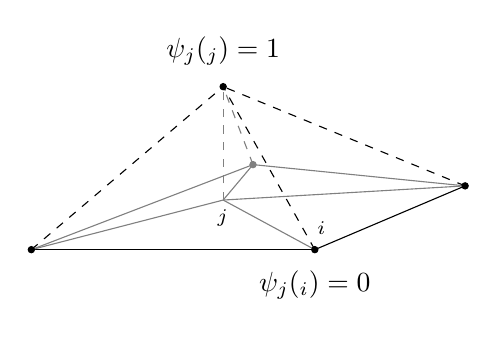
\begin{tikzpicture}[scale=0.9, z={(.707,.3)}]
    % (2,2,1) is top
    \draw[style=dashed] (0,0,0) -- (2,2,1); % to top from left
    \draw[style=dashed] (4,0,0) -- (2,2,1); %   ...  from front
    \draw[style=dashed] (4,0,3) -- (2,2,1); %   ...  from right
    \draw[color=gray, style=dashed] (0.3,0,4) -- (2,2,1); % from back
    \draw[color=gray, style=dashed] (2,0.4,1) -- (2,2,1); % from middle
    % draw base
    \draw (0,0,0) -- (4,0,0);
    \draw (4,0,0) -- (4,0,3);
    \draw[color=gray] (0,0,0) -- (0.3,0,4);
    \draw[color=gray] (0.3,0,4) -- (4,0,3);
    \draw[color=gray] (0,0,0) -- (2,0.4,1);
    \draw[color=gray] (2,0.4,1) -- (4,0,3);
    \draw[color=gray] (4,0,0) -- (2,0.4,1);
    \draw[color=gray] (2,0.4,1) -- (0.3,0,4);
    % draw \psi_j at nodes
    \filldraw (2,2,1) circle (1.25pt);
    \draw (2,2.5,1) node {$\psi_j(\bx_j)=1$};
    \draw (2,0.15,1) node {$\bx_j$};
    \filldraw (0,0,0) circle (1.25pt);
    \filldraw (4,0,0) circle (1.25pt);
    \draw (4,-0.5,0) node {$\psi_j(\bx_i)=0$};
    \draw (4.1,0.3,0) node {$\bx_i$};
    \filldraw (4,0,3) circle (1.25pt);
    \filldraw[color=gray] (0.3,0,4) circle (1.25pt);
\end{tikzpicture}


\caption{Hat functions $\psi_j$.}
\label{fig:un:hatfunction}
\end{marginfigure}

The FEM itself can now be stated.  It seeks $u^h\in S_{g}^h$ so that \eqref{eq:un:poissonweak} holds for all $v^h\in S_{0}^h$.  By linearity it suffices to consider only a basis of test functions $S_{0}^h$, so we require
\begin{equation}
\int_\Omega a(u^h) \grad u^h \cdot \grad \psi_i = \int_\Omega f(u^h) \psi_i + \int_{\partial_N\Omega} g_N \psi_i \label{eq:un:weakformhat}
\end{equation}
for all $i$ such that $\bx_i \notin \partial_D \Omega$.

On the other hand we may expand $u^h$ using $N-n_D$ unknown coefficients $u_j\in\RR$:
\begin{equation}
u^h(x,y) = \hat g_D(x,y) + \sum_{\bx_j \notin \partial_D \Omega} u_j\, \psi_j(x,y). \label{eq:un:uhexpand}
\end{equation}
The coefficients $u_j$ in \eqref{eq:un:uhexpand} are the unknowns.

Given the triangulation $\mathcal{T}_h$ of $\Omega$ and the data of the problem, namely the functions $a$, $f$, $g_D$, and $g_N$, the complete specification of the FEM solution $u^h$ is given by equations \eqref{eq:un:hatgdefine}, \eqref{eq:un:weakformhat}, and \eqref{eq:un:uhexpand}.  This FEM problem can be shown to be well-posed, in the linear case at least, by the same theory that applies to the continuum problem.

As a next step in the linear case it is common to write system \eqref{eq:un:weakformhat} and \eqref{eq:un:uhexpand} in matrix-vector form as $A \bu = \bb$, and then to assemble the \emph{stiffness matrix} $A$ \citep{Elmanetal2005}.  However, as said earlier, we will not assemble a matrix until we have an initial, verified numerical solution.  Following the pattern established since Chapter \ref{chap:nl}, we first implement equation \eqref{eq:un:weakformhat} as a residual function $\bF(\bu)$, a \PETSc \pSNES call-back, in which the input $\bu$ is the representation of $u^h$ as a vector of nodal values.  In evaluating $\bF$ we use \eqref{eq:un:uhexpand} to get point values of $u^h$, and its gradient $\grad u^h$, on the interior of triangles.  These point values allow quadrature, similar to that in Chapter \ref{chap:of}, to approximate the integrals in \eqref{eq:un:weakformhat}.  Implementing a residual in the linear case is mathematically equivalent to assembling $A$ and $\bb$, but the residual-evaluation code requires no direct contact with a \PETSc \pMat object.  Our solution can then be tested for correctness with a finite-differenced Jacobian (Chapter \ref{chap:nl}).  Once it is shown to work correctly, via comparison to an exact solution, then we re-consider matrix assembly for the Jacobian.

Before the code can be written we need to be more specific about what \eqref{eq:un:weakformhat} says on each element, and we need to read a triangular mesh into \PETSc data structures.


\section{Assembly of the residual equations}

In expression \eqref{eq:un:uhexpand}, $N-n_D$ values $\{u_j\}$ determine the FEM solution $u^h$.  However, it will be easier to write code if we \emph{increase} the size of the resulting nonlinear system up to dimension $N$ by including the nodal values in the Dirichlet boundary as unknowns:
\begin{equation}
\bu = \{u_j\}_{j=0}^{N-1} \in \RR^N  \label{eq:un:unknowns}
\end{equation}
To enforce the boundary conditions, the components of the residual corresponding to the Dirichlet boundary must be zero:
\begin{equation}
F_i(\bu) = u_i - g_D(\bx_i) \qquad \text{ if } \bx_i \in \partial_D\Omega.  \label{eq:un:dirichletresiduals}
\end{equation}

Triangulation $\mathcal{T}_h$ covers $\Omega$ with non-overlapping triangles, so we can write integral \eqref{eq:un:weakformhat} as a sum over elements.  In fact, for each $k=0,\dots,K-1$ let
\begin{equation}
F_i^k(\bu) = \int_{\triangle_k} a(u^h) \grad u^h \cdot \grad \psi_i - f(u^h) \psi_i.  \label{eq:un:elementweakform}
\end{equation}
Suppose $n_N$ is the number of segments (edges) which are in the Neumann boundary.  For each segment $s_\nu$, $\nu=0,\dots,n_N-1$, let
\begin{equation}
\varphi_i^\nu = \int_{s_\nu} g_N \psi_i.  \label{eq:un:segmentweakform}
\end{equation}
(Note that $\varphi_i^\nu$ does \emph{not} depend on the solution $u^h$.)  Then \eqref{eq:un:weakformhat} becomes the statement that the following residual components are zero:
\begin{equation}
F_i(\bu) = \sum_{k=0}^{K-1} F_i^k(\bu) - \sum_{\nu=0}^{n_N-1} \varphi_i^\nu  \qquad \text{ if } \bx_i \notin \partial_D\Omega. \label{eq:un:elementwisesum}
\end{equation}
Together, equations \eqref{eq:un:dirichletresiduals} and \eqref{eq:un:elementwisesum} form a (generally) nonlinear system, of dimension $N$, which the \pSNES is asked to solve:
\begin{equation}
\bF(\bu)=0. \label{eq:un:fullsystem}
\end{equation}

Observe that $n_D$ is the number of \emph{nodes} in the Dirichlet boundary, whereas $n_N$ is the number of \emph{segments} in the Neumann boundary.  The former are degrees of freedom, while the latter are domains of integration.

Because the support of the hat function $\psi_i$ only overlaps with a few triangles $\triangle_k$, for each $i$ only a few values $F_i(\bu)$ and $\varphi_i^\nu$ are nonzero.  Also, only a few nodal values $\bu=\{u_j\}$ enter into $F_i^k(\bu)$, namely those values $u_j$ such that the support of $\psi_j$ overlaps with $\psi_i$.  These facts make \eqref{eq:un:fullsystem} a sparse nonlinear system.

We will compute the element integrals \eqref{eq:un:elementweakform} by referring $\triangle_k$ to a reference triangle $\triangle_\ast$ with vertices $(0,0),\,(1,0),\,(0,1)$, as shown in Figure \ref{fig:isoparametric}.  (In Chapter \ref{chap:of} we did something similar for quadrilaterals.)  If $\triangle_k$ has vertices $(x_0,y_0),\,(x_1,y_1),\,(x_2,y_2)$ then the linear map from $\triangle_\ast$ to $\triangle_k$ is
\begin{align}
x(\xi,\eta) &= x_0 + (x_1-x_0) \xi + (x_2-x_0) \eta, \label{eq:un:trianglemap} \\
y(\xi,\eta) &= y_0 + (y_1-y_0) \xi + (y_2-y_0) \eta. \notag
\end{align}
The Jacobian determinant of this map, needed for integrating, is constant on each element.  Its magnitude $2|\triangle_k|$ is the ratio of the triangle areas.

\begin{marginfigure}
\begin{tikzpicture}[scale=1.1,
    decoration={
      markings,
      mark=at position 1 with {\arrow[scale=1.8,gray]{latex}};
    }]
% left x,y axes
    \draw[->, gray, very thin] (1.5,0) -- (4.0,0);
    \draw[->, gray, very thin] (2,-0.5) -- (2,2.4);
    \draw (4.1,-0.1) node {$x$};
    \draw (1.9,2.4) node {$y$};
    \filldraw (1.7,1) circle (1.25pt);    % (x_0,y_0)
    \filldraw (3.5,-0.3) circle (1.25pt); % (x_1,y_1)
    \filldraw (3.0,2.0) circle (1.25pt);  % (x_2,y_2)
    \draw (1.4,1.3) node {$(x_0,y_0)$};
    \draw (3.5,-0.6) node {$(x_1,y_1)$};
    \draw (3.0,2.3) node {$(x_2,y_2)$};
    \draw[line width=1pt] (1.7,1) -- (3.5,-0.3) -- (3.0,2.0) -- cycle;
    \draw (2.7,1.0) node {$\triangle_k$};
% right xi,eta axes
    \draw[->, gray, very thin] (4.6,0) -- (6.6,0);
    \draw[->, gray, very thin] (5,-0.4) -- (5,2.0);
    \draw (6.7,-0.1) node {$\xi$};
    \draw (4.9,2.05) node {$\eta$};
    \filldraw (5,0) circle (1.25pt);  % (0,0)
    \filldraw (6,0) circle (1.25pt);  % (1,0)
    \filldraw (5,1) circle (1.25pt);  % (0,1)
    \draw (5.2,-0.3) node {$0$};
    \draw (6.2,0.2) node {$1$};
    \draw (5.2,1.1) node {$2$};
    \draw[line width=1pt] (5,0) -- (6,0) -- (5,1) -- cycle;
    \draw (5.3,0.3) node {$\triangle_\ast$};
% arrows connecting nodes
    \draw[gray, postaction={decorate}] (5,0) -- (1.7,1.03);
    \draw[gray, postaction={decorate}] (6,0) -- (3.5,-0.3);
    \draw[gray, postaction={decorate}] (5,1) -- (3.0,2.0);
\end{tikzpicture}


\caption{Mapping of a triangle $\triangle_k$ from the reference triangle $\triangle_\ast$.}
\label{fig:isoparametric}
\end{marginfigure}

On $\triangle_\ast$ any linear function is a linear combination of three local (nodal) basis functions:
\begin{equation}
\chi_0(\xi,\eta) = 1-\xi-\eta, \qquad \chi_1(\xi,\eta) = \xi, \qquad \chi_2(\xi,\eta) = \eta. \label{eq:un:chiformulas}
\end{equation}
If $\bx_i\in\overline{\triangle_k}$ then $\psi_i$ satisfies
\begin{equation}
\psi_i(x(\xi,\eta),y(\xi,\eta)) = \chi_\ell(\xi,\eta) \label{eq:un:psichimap}
\end{equation}
for all $(\xi,\eta)\in\triangle_\ast$, where vertex $\ell \in \{0,1,2\}$ of $\triangle_\ast$ maps to $\bx_i$.

Recalling both the change-of-variables formula for integrals and the chain rule, we can write
\begin{equation}
F_i^k(\bu) = 2 |\triangle_k| \int_{\triangle_\ast} H_\ell^k(\bu,\xi,\eta)\,d\xi\,d\eta \label{eq:un:elementintegralreference}
\end{equation}
where the integrand is
\begin{equation}
H_\ell^k(\bu,\xi,\eta) = \left[a(u^h) \grad u^h \cdot \grad \psi_i - f(u^h) \psi_i\right]_{\triangle_\ast}.  \label{eq:un:elementintegrand}
\end{equation}
Here vertex $\ell$ of $\triangle_\ast$ corresponds to the node $\bx_i$.  Note that ``$\grad$'' in \eqref{eq:un:elementintegrand} refers to derivatives in variables $x,y$.  Exercises \ref{chap:un}.\ref{exer:un:gradientdetails} and \ref{chap:un}.\ref{exer:un:elementintegranddetails} addresses the remaining details implicit in \eqref{eq:un:elementintegralreference} and \eqref{eq:un:elementintegrand}.

As in Chapter \ref{chap:of}, integrals \eqref{eq:un:elementintegralreference} are approximated using quadrature.  Generally, if there are $Q$ quadrature points $(\xi_q,\eta_q) \in \triangle_\ast$ with weights $w_q$ then
\begin{equation}
F_i^k(\bu) \approx 2 |\triangle_k| \sum_{q=0}^{Q-1} w_q H_\ell^k(\bu,\xi_q,\eta_q). \label{eq:un:elementquadraturereference}
\end{equation}
We use symmetric quadrature rules constructed for the reference triangle $\triangle_\ast$ \citep{Dunavant1985}.  (Unsymmetric quadrature rules based on tensor products of one-dimensional integrals \citep{KarniadakisSherwin2013} are an alternative.)  Table \ref{tab:un:quadrature} shows the degree $1,2,3$ Gaussian rules with $Q=1,3,4$ points, respectively (Exercise \ref{chap:un}.\ref{exer:un:checkquadrature}).  Note that the sum of the weights is $1/2$ because $|\triangle_\ast|=1/2$.

\begin{table}[h]
\vspace{0.1in}

\begin{tabular}{lccc}
degree & $Q$ & weights $w_q$ & nodes $(\xi_q,\eta_q)$ \\ \hline
$1$ & $1$ & $1/2$ & $(1/3,1/3)$ \\ \hline
$2$ & $3$ & \begin{tabular}{c}
            $1/6$ \\
            $1/6$ \\
            $1/6$
            \end{tabular} & \begin{tabular}{c}
            $(1/6,1/6)$ \\
            $(2/3,1/6)$ \\
            $(1/6,2/3)$
            \end{tabular} \\ \hline
$3$ & $4$ & \begin{tabular}{c}
            $-27/96$ \\
            $25/96$ \\
            $25/96$ \\
            $25/96$
            \end{tabular} & \begin{tabular}{c}
            $(1/3,1/3)$ \\
            $(1/5,1/5)$ \\
            $(3/5,1/5)$ \\
            $(1/5,3/5)$
            \end{tabular}
\end{tabular}

\vspace{0.1in}
\caption{Symmetric quadrature rules with $Q$ points on the reference triangle $\triangle_\ast$.  See \eqref{eq:un:elementquadraturereference}.} \label{tab:un:quadrature}
\end{table}

For the Neumann boundary contributions we use the midpoint rule; compare Exercise \ref{chap:un}.\ref{exer:un:gaussneumann}.  Observe that hat function $\psi_i$ has value $1/2$ at the midpoint of an edge incident to $\bx_i$.  If $(x_m,y_m)$ is this midpoint, $|s_\nu|$ is the length of segment $s_\nu$, and $\bx_i\in \overline{s_\nu}$ then
\begin{equation}
\varphi_i^\nu \approx g_N(x_m,y_m) \psi_i(x_m,y_m) |s_\nu| = \frac{1}{2} |s_\nu|\, g_N(x_m,y_m). \label{eq:un:segmentquadrature}
\end{equation}
Otherwise, if $\bx_i \notin \overline{s_\nu}$, then $\varphi_i^\nu=0$.


\section{Example problems}

Now let us set up some simple cases with known exact solutions.  The three cases test the implementation of the PDE and the boundary conditions.  Two problems are linear and one is nonlinear.  Our goal for these problems is that the measured numerical errors from the FEM will only converge at the theoretical rate $O(h^2)$ \citep{Elmanetal2005} for all cases if our implementation is correct.

\begin{figure}
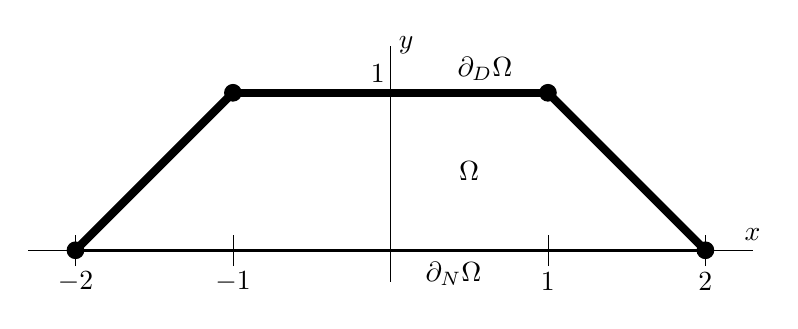
\begin{tikzpicture}[scale=2.000000]
% originally created, in part, by script tri2tikz.py command line:
%   tri2tikz.py --polyonly --nodesize 1.0 --scale 2.0 ../c/ch8/meshes/trap tmp/trap.tikz
% with by-hand edits
  \draw[thin] (0.0,-0.2) -- (0.0,1.3);
  \draw[thin] (-2.3,0.0) -- (2.3,0.0);
  \node at (2.3,0.1) {$x$};
  \node at (0.1,1.3) {$y$};
  \node at (0.5,0.5) {$\Omega$};
  \node at (-0.08,1.12) {$1$};
  \draw[very thin] (-2.0,-0.1) -- (-2.0,0.1);
  \node at (-2.0,-0.2) {$-2$};
  \draw[very thin] (-1.0,-0.1) -- (-1.0,0.1);
  \node at (-1.0,-0.2) {$-1$};
  \draw[very thin] (1.0,-0.1) -- (1.0,0.1);
  \node at (1.0,-0.2) {$1$};
  \draw[very thin] (2.0,-0.1) -- (2.0,0.1);
  \node at (2.0,-0.2) {$2$};
  \node at (0.4,-0.15) {$\partial_N \Omega$};
  \node at (0.6,1.15) {$\partial_D \Omega$};
  \draw[line width=3.0pt] (2.000000,0.000000) -- (1.000000,1.000000);
  \draw[line width=3.0pt] (1.000000,1.000000) -- (-1.000000,1.000000);
  \draw[line width=3.0pt] (-1.000000,1.000000) -- (-2.000000,0.000000);
  \draw[line width=1.25pt] (-2.000000,0.000000) -- (2.000000,0.000000);
  \filldraw (2.0,0.0) circle (1.5pt);
  \filldraw (1.0,1.0) circle (1.5pt);
  \filldraw (-1.0,1.0) circle (1.5pt);
  \filldraw (-2.0,0.0) circle (1.5pt);
\end{tikzpicture}

\caption{Exact solution cases $0$ and $1$ solve Poisson equations on a trapezoidal region $\Omega$.  Boundary subsets $\partial_D\Omega$, $\partial_N \Omega$ are as indicated.  See \texttt{trap.poly} in Code \ref{code:trappoly}.}
\label{fig:un:trap}
\end{figure}

All three cases are based on the same manufactured solution
\begin{equation}
  u_{\text{exact}}(x,y) = 1 - y^2 - \frac{1}{4} y^4. \label{eq:un:exactsolution}
\end{equation}
This formula also computes the Dirichlet boundary values $g_D(x,y)$ in all cases, but other details are case-specific:
\begin{itemize}
\item[case $0$:] \emph{Linear}.  Use Figure \ref{fig:un:trap} boundary conditions.  Noting $\partial u_{\text{exact}}/\partial n = -\partial u_{\text{exact}}/\partial y = 0$ on the Neumann boundary $\partial_N \Omega = \{y=0\}$, let $g_N=0$.  Let $a=1$ and determine $f$ by differentiating the exact solution, so that $f(x,y) = 2 + 3 y^2$.
\item[case $1$:] \emph{Nonlinear}.  Again use Figure \ref{fig:un:trap} boundary conditions and $g_N=0$.  However, let $a(u) = 1+u^2$ and determine $f(u)$ by differentiation.
\item[case $2$:] \emph{Non-homogeneous Neumann}.  Use Figure \ref{fig:un:trapneu} boundary conditions.  Let $a$, $f$ be the same as in case $0$.  Determine the (non-zero) value $g_N$ by differentiating $u_{\text{exact}}$ along the Neumann boundary, a line segment with outward unit normal vector $\bn = \left<1/1\right>/\sqrt{2}$.
\end{itemize}
See \texttt{c/\CODELOC cases.h} (not shown) for all remaining details.

\begin{figure}
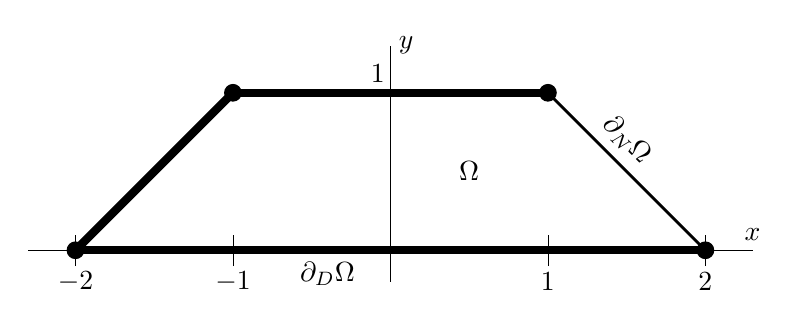
\begin{tikzpicture}[scale=2.000000]
% originally created, in part, by script tri2tikz.py command line:
%   tri2tikz.py --polyonly --nodesize 1.0 --scale 2.0 ../c/ch8/meshes/trap tmp/trap.tikz
% with by-hand edits
  \draw[thin] (0.0,-0.2) -- (0.0,1.3);
  \draw[thin] (-2.3,0.0) -- (2.3,0.0);
  \node at (2.3,0.1) {$x$};
  \node at (0.1,1.3) {$y$};
  \node at (0.5,0.5) {$\Omega$};
  \node at (-0.08,1.12) {$1$};
  \draw[very thin] (-2.0,-0.1) -- (-2.0,0.1);
  \node at (-2.0,-0.2) {$-2$};
  \draw[very thin] (-1.0,-0.1) -- (-1.0,0.1);
  \node at (-1.0,-0.2) {$-1$};
  \draw[very thin] (1.0,-0.1) -- (1.0,0.1);
  \node at (1.0,-0.2) {$1$};
  \draw[very thin] (2.0,-0.1) -- (2.0,0.1);
  \node at (2.0,-0.2) {$2$};
  \node at (-0.4,-0.15) {$\partial_D \Omega$};
  \node[rotate=-45] at (1.5,0.7) {$\partial_N \Omega$};
  \draw[line width=1.0pt] (2.000000,0.000000) -- (1.000000,1.000000);
  \draw[line width=3.0pt] (1.000000,1.000000) -- (-1.000000,1.000000);
  \draw[line width=3.0pt] (-1.000000,1.000000) -- (-2.000000,0.000000);
  \draw[line width=3.0pt] (-2.000000,0.000000) -- (2.000000,0.000000);
  \filldraw (2.0,0.0) circle (1.5pt);
  \filldraw (1.0,1.0) circle (1.5pt);
  \filldraw (-1.0,1.0) circle (1.5pt);
  \filldraw (-2.0,0.0) circle (1.5pt);
\end{tikzpicture}

\caption{Case $2$ uses the same region as in cases $0$ and $1$, but with different boundary conditions.  See \texttt{c/\CODELOC meshes/trapneu.poly} (not shown).}
\label{fig:un:trapneu}
\end{figure}


\section{Triangulations from \Triangle}

\PETSc does not include tools for triangulating regions of the plane, that is, for the initial generation of an unstructured mesh.  We use the widely-available \Triangle\sidenote{See \href{http://www.cs.cmu.edu/~quake/triangle.html}{www.cs.cmu.edu/$\sim$quake/ triangle.html} for documentation.} software \citep{Shewchuk1996} for this task.  While \Triangle is limited to 2D, the ASCII files it generates have straightforward details.

\inputwhole{../c/\CODELOC/meshes/trap.poly}{\CODELOC meshes/trap.poly}{A description of the boundary polygon in Figure \ref{fig:un:trap}, suitable for reading by \Triangle.}{code:trappoly}

\Triangle takes as input an ASCII file describing a polygonal region $\Omega$.  This file contains integer flags (``markers'') which classify the vertices or segments on the boundary.  For example, the input file \texttt{trap.poly} (Code \ref{code:trappoly}) generates the polygon shown in Figure \ref{fig:un:trap}.

The triangulation shown in Figure \ref{fig:un:trapone} came from applying \Triangle to \texttt{trap.poly}, as follows.  We ask for a polygon output file (option \texttt{-p}), relatively-uniform triangles (\texttt{-q} for ``quality-checked''),\sidenote{I.e.~with no interior angles less than $20^\circ$ \citep{Shewchuk1996}.} and triangles with a maximum area (\texttt{-a}) of $0.5$:
\begin{cline}
$ cd c/ch7/meshes
$ triangle -pqa0.5 trap
\end{cline}
%$
The command generates three ASCII files, \texttt{trap.1.node}, \texttt{trap.1.ele}, and \texttt{trap.1.poly}; see Codes \ref{code:traponenode}--\ref{code:traponepoly}.  They define the new node locations, elements (triples of nodal indices), and segments in the polynomial boundary (pairs of nodal indices), respectively.  As seen in Figure \ref{fig:un:trapone}, this triangulation has $N=8$ nodes, $K=6$ elements, $P=8$ boundary segments, $n_D=5$ Dirichlet nodes, and $n_N=4$ segments in the Neumann boundary.

\begin{figure}
\input{tmp/trap.1.tikz}
\caption{The triangulation described by \texttt{trap.1.\{node,ele,poly\}}.}
\label{fig:un:trapone}
\end{figure}

\inputwhole{misc/trap.1.node}{\CODELOC meshes/trap.1.node}{Node locations and nodal boundary flags for the mesh in Figure \ref{fig:un:trapone}.}{code:traponenode}

By giving value ``$2$'' to the Dirichlet nodes in the original \texttt{trap.poly} input, and because \Triangle itself uses ``$0$'' for non-boundary and ``$1$'' for otherwise un-flagged boundary nodes, we have this boundary flag scheme:
\begin{itemize}
\item[$0=$] interior node,
\item[$1=$] Neumann boundary segment (or node), and
\item[$2=$] Dirichlet boundary node (or segment).
\end{itemize}
In \texttt{trap.1.node} observe that additional nodes have been added to the boundary.

\inputwhole{misc/trap.1.ele}{\CODELOC meshes/trap.1.ele}{Element index triples for the mesh in Figure \ref{fig:un:trapone}.}{code:traponeele}

We will test the FEM on a sequence of refined grids generated by \Triangle.  For an example, the command
\begin{cline}
$ triangle -rpqa0.1 trap.1
\end{cline}
%$
generates ASCII files \texttt{trap.2.\{node,ele,poly\}} with $N=33$ nodes, $K=33$ elements, and $P=19$ boundary segments (Figure \ref{fig:un:traptwo}).  Refinement (\texttt{-r}) here means that \emph{nodes} in the \texttt{trap.1} files are retained, but there is no simple inclusion relationship for the interior edges or triangles.  We also see that the symmetry of the \texttt{trap.1} mesh was merely fortuitous as symmetries in the input polygon are not preserved by the \Triangle algorithms.

\inputwhole{misc/trap.1.poly}{\CODELOC meshes/trap.1.poly}{Refined polygon, including segment boundary flags, for the mesh in Figure \ref{fig:un:trapone}.}{code:traponepoly}

\begin{figure}
\input{tmp/trap.2.tikz}
\caption{A refined triangulation.}
\label{fig:un:traptwo}
\end{figure}

\Triangle includes a mesh visualization tool.  The command
\begin{cline}
$ showme trap
\end{cline}
%$
displays all of the generated triangulation levels (i.e.~\texttt{trap.\{1,2\}.\{node,ele,poly\}}).


\section{Loading the mesh into \PETSc \pVecs and \pISs}

Our plan is to traverse the elements $\triangle_k \in \mathcal{T}_h$, and the Neumann boundary segments $s_\nu$, to compute \eqref{eq:un:elementquadraturereference} and \eqref{eq:un:segmentquadrature}.  The traversal is reasonably fast if the mesh data are read from \PETSc binary format files.  Thus we convert the \Triangle-generated ASCII files into \pVec and \pIS types stored in binary by using a Python script \texttt{tri2petsc.py}.

Note that there are two kinds of ``data'' to describe a triangulation, \emph{geometrical} and \emph{topological}.  The geometry is simply the nodal locations, pairs of real numbers for each node.  We store these coordinates in a length $2N$ sequential \pVec.  For the topology we know which elements (triangles) are incident to which nodes (vertices) only using integer indices.  Each element is given by a triple of integers, node indices in the range $0,\dots,N-1$.  Similarly, a segment of the polygonal boundary is simply a pair of indices for its endpoint nodes.

The \PETSc \pIS ``index set'' type is convenient for storing indices.  The reader may for now regard an \pIS simply as an ``integer-valued \pVec.''\sidenote{In this Chapter we do not exploit the ``main purpose'' of an \pIS, namely in distributed (multi-process) indexing.}  The \pIS storing the element index triples holds $3K$ integers and the one for boundary segments holds $2P$ integers.

Some care is needed in recording the Dirichlet and Neumann parts of the boundary.  First, one cannot tell if an edge is a boundary segment just from whether the endpoints are in the boundary.\sidenote{For example, the edge from node 5 to node 7 in Figure \ref{fig:un:number-mesh} is not a boundary segment.}  Second, even if the endpoints of a boundary segment are in the (closed) Dirchlet boundary, the segment itself might be in the (relatively-open) Neumann boundary.  Therefore, despite the apparent redundancy, we will separately store flags for the \emph{nodes}, indicating whether they are interior ($0$) or Neumann boundary ($1$) or Dirichlet boundary ($2$), and for the \emph{segments} on the boundary, either $1$ for Neumann or $2$ for Dirichlet.  This scheme is already shown in \Triangle outputs above (Codes \ref{code:traponenode}--\ref{code:traponepoly}).  Two more \pISs are used to store boundary flags.

Thus the Python script \texttt{tri2petsc.py} (not shown) reads three files in \Triangle-generated ASCII format, as described above, with extensions \texttt{.node,.ele,.poly}.  Then it writes two files in \PETSc binary format with extensions \texttt{.vec,.is}.  The first output file holds a \pVec with the node coordinates.  The second output file holds four \pISs (element triples, nodal boundary flags, boundary segment pairs, and boundary segment flags).

Let's try it out.  Because \texttt{tri2petsc.py} uses Python modules from the \PETSc source directory, we generate some symbolic links before converting:
\begin{cline}
$ cd c/ch7/
$ ln -s ~/petsc/bin/petsc_conf.py
$ ln -s ~/petsc/bin/PetscBinaryIO.py
$ ./tri2petsc.py meshes/trap.1 meshes/trap.1
\end{cline}
This generates files \texttt{meshes/trap.1.\{vec,is\}}.

\cinputpart{um.h}{\CODELOC}{\texttt{UM} is an unstructured-mesh data type.}{I}{//STARTSTRUCT}{//ENDSTRUCT}{code:umstruct}

Our C code is, for the first time in the book, designed in a modular, instead of monolithic, way.  We separate the representation of the mesh, and associated file input/output functions, from the tasks of computing the residual and setting up the \PETSc solver.  The reader should examine the following files in \texttt{c/ch7/}:
\begin{itemize}
\item \texttt{um.h} and \texttt{um.c}:\quad  Declares a simple unstructured-mesh ``object'' \texttt{UM} as a C \texttt{struct} and provides an interface for it.  The major functions read a mesh from binary files and view it.
\item \texttt{cases.h}:\quad  Exact solutions and boundary conditions for the problem cases above.  (Note shown.)
\item \texttt{unfem.c}:\quad  Contains a residual evaluation function.  Also reads options, calls functions from \texttt{cases.h} to set boundary conditions, calls functions from \texttt{um.h} to read the mesh, sets up a \pSNES solver object, runs the solver, and reports the numerical error.
\end{itemize}

The \texttt{UM} (``unstructured mesh'') \texttt{struct} is declared in Code \ref{code:umstruct}.  The ``methods'' for this ``object'' are declared in Code \ref{code:umdeclare}.  \texttt{UMInitialize()} should be called before anything else, and \texttt{UMDestroy()} last.  Function \texttt{UMReadNodes()} should be called before \texttt{UMReadISs()}; these load binary data using \PETSc functions  \texttt{VecLoad()} and \texttt{ISLoad()}, respectively.  The (tedious) implementations of these functions in \texttt{c/ch7/um.c} are not shown.

\cinputpart{um.h}{\CODELOC}{The ``methods'' for the \texttt{UM} unstructured-mesh data type.}{II}{//STARTDECLARE}{//ENDDECLARE}{code:umdeclare}

Despite our attempt at modularity, our representation of an unstructured mesh is deliberately simple and even naive.  It motivates the Chapter \ref{chap:dp} coverage of \PETSc support for unstructured meshes.


\section{Initial implementation}

With an unstructured mesh in hand we can return to implementing the FEM.  We build a \pSNES-using code\sidenote{In terms of \PETSc objects and calls, \texttt{unfem.c} is similar to \texttt{ecjac.c} in Chapter \ref{chap:nl} in the sense that there is no \PETSc-supported grid topology.} which works, called \texttt{c/\CODELOC unfem.c}.  The most important parts are a residual-computation function \texttt{FormFunction()} and a \texttt{main()} function.  Figure \ref{fig:un:unfemstack} shows the structure, including the approximate-Jacobian \texttt{FormPicard()} which we implement later.  Extracts from \texttt{c/ch7/unfem.c}, displaying all essentials of the initial implementation, are shown in Codes \ref{code:unfemctx}--\ref{code:unfemelementresiduals}.

\begin{figure}
\begin{tikzpicture}[scale=0.8,
                    >={Latex[length=2mm]},
  component/.style={
     rectangle,draw,fill=white,align=center,line width=1pt},
  userfcn/.style={
     rounded corners,draw,fill=white,draw,align=center,line width=1pt,font={\itshape,\normalsize}}]

\draw[line width=1pt] (3,7) node[userfcn,minimum width=105mm] (usercode) {user code \\ \vspace{15mm}};

\draw[line width=1pt] (0,7.2) node[userfcn] (rescode) {residual \emph{\texttt{FormFunction()}}};
\draw[line width=1pt] (5.2,6.2) node[userfcn] (jaccode) {approximate Jacobian \emph{\texttt{FormPicard()}}};

\draw[line width=1pt] (-1,4) node[component] (snes) {\complabel{\pSNES}{nonlinear solver}};
\draw[line width=1pt] (-1,2) node[component] (ksp)  {\complabel{\pKSP}{linear solver}};
\draw[line width=1pt] (-1,0) node[component] (pc)   {\complabel{\pPC}{preconditioner}};

\draw[line width=1pt] (2,2) node[component] (matj)   {\usedlabel{\pMat}{Jacobian}};
\draw[line width=1pt] (3.5,0) node[component] (vecs)   {\pVecs \\ \footnotesize  \emph{node coordinates, solution}};
\draw[line width=1pt] (7.5,0) node[component] (iss)   {\pISs \\ \footnotesize  \emph{indices, bdry flags}};

\path
   ([xshift=-10em]usercode.south) edge[->] node {} (snes)
   ([xshift=0em]usercode.south) edge[->] node {} ([xshift=2em]vecs.north)

   (rescode.south) edge[->,bend left] node {} (vecs.north)
   ([xshift=-2em]rescode.south) edge[->] node {} (iss.north)

   (jaccode.south) edge[->] node {} (matj)
   ([xshift=2em]jaccode.south) edge[->] node {} ([xshift=4em]vecs.north)
   ([xshift=4em]jaccode.south) edge[->] node {} ([xshift=2em]iss.north)

   (snes) edge node {} (ksp)
   (ksp) edge node {} (pc);
\end{tikzpicture}
\caption{The structure of \texttt{unfem.c}.}
\label{fig:un:unfemstack}
\end{figure}

So that the residual-evaluation function \texttt{FormFunction()} has access to functions $a$, $f$, $g_D$, $g_N$ in FEM \eqref{eq:un:weakformhat}, we define a solution context \texttt{unfemCtx} in Code \ref{code:unfemctx}.  This \texttt{struct} also includes the mesh, namely a pointer to a \texttt{UM} instance.

\cinputpart{unfem.c}{\CODELOC}{Context for solving FEM \eqref{eq:un:weakformhat}, \eqref{eq:un:uhexpand} on an unstructured mesh.}{I}{//STARTCTX}{//ENDCTX}{code:unfemctx}

Only an extract of the \texttt{main()} function is displayed here (Code \ref{code:unfemmain}).  We do not show the first actions of \texttt{main()}, which are to read options and choose appropriate functions $a,f,g_D,g_N$ for the problem case.  The portion shown in Code \ref{code:unfemmain} starts with reading a mesh from \PETSc binary files via calls to the ``methods'' of the \texttt{UM} object.  Then \pVecs are allocated and the \pSNES solver is configured.  We set a call-back to \texttt{FormFunction()} by using \texttt{SNESSetFunction()}.

\cinputpart{unfem.c}{\CODELOC}{An extract of \texttt{main()}: read the mesh, set-up \pVecs, configure \pSNES, and reset the default \pKSP and \pPC for our symmetric, positive-definite problem.}{II}{//STARTMAININITIAL}{//ENDMAININITIAL}{code:unfemmain}

Though we do not, for now, need to do any work to assemble it, the symmetry and positive-definiteness of the Jacobian matrix is already relevant here.  In the linear case, in which $\partial a/\partial u=0$ and $\partial f/\partial u=0$ in \eqref{eq:un:poissonweak}, the Jacobian $J_{ij} = \partial F_i/\partial u_j$ is symmetric and positive-definite.  Thus we reset the default \pKSP and \pPC types to conjugate gradient (CG) and incomplete-Cholesky (ICC).  This is done in Code \ref{code:unfemmain} by first getting a pointer to the \pKSP inside the \pSNES---see Figure \ref{fig:un:unfemstack}---and then setting its type.  Getting a pointer to the \pPC inside the \pKSP then allows setting the \pPC type as well.

The extract in Code \ref{code:unfemmain} also shows that an analytical Jacobian \pMat \texttt{A} is allocated, and a \pSNES call-back is set with \texttt{SNESSetJacobian()}.  These actions are ignored if \texttt{-snes\_fd} or \texttt{-snes\_mf} are used, as we do initially.

\cinputpart{unfem.c}{\CODELOC}{Our FEM uses local basis functions $\chi_\ell$ and some quadrature tools.}{III}{//STARTFEM}{//ENDFEM}{code:unfemfem}

Code \ref{code:unfemfem} shows FEM details (``tools'') appearing in \texttt{c/ch7/unfem.c}.  For example, the first few displayed lines correspond to equation \eqref{eq:un:chiformulas} for the local basis functions $\chi_\ell(\eta,\xi)$.  There are also functions to evaluate the gradients $\grad \chi_\ell$ and linear combinations $\sum_\ell v_\ell \chi_\ell$.  The remaining lines define arrays for the quadrature rules in Table \ref{tab:un:quadrature}.

The residual $\bF(\bu)$ is evaluated by \texttt{FormFunction()}.  It is shown in Codes \ref{code:unfembdryresiduals}--\ref{code:unfemelementresiduals}.  Note that input \texttt{Vec u} is accessed using a \texttt{const double *} pointer and \texttt{VecGetArrayRead()}, while \texttt{Vec F} is an output accessed using a \texttt{double *} pointer and \texttt{VecGetArray()}.  Function \texttt{UMGetNodeCoordArrayRead()} (Code \ref{code:umdeclare}) gives a pointer to an array of \texttt{Node}s (Code \ref{code:umstruct}).  When accessing indices we use \texttt{ISGetIndices()}.  All of these \texttt{Get} functions have a matching \texttt{Restore}.

\cinputpart{unfem.c}{\CODELOC}{\texttt{FormFunction()} first evaluates \eqref{eq:un:dirichletresiduals} and \eqref{eq:un:segmentweakform} for the boundary contributions.}{IV}{//STARTBDRYRESIDUALS}{//ENDBDRYRESIDUALS}{code:unfembdryresiduals}

\cinputpart{unfem.c}{\CODELOC}{Next, \texttt{FormFunction()} traverses the elements to compute residuals \eqref{eq:un:elementweakform}.}{V}{//STARTELEMENTRESIDUALS}{//ENDELEMENTRESIDUALS}{code:unfemelementresiduals}

\texttt{FormFunction()} loops through all $N$ nodes and computes \eqref{eq:un:dirichletresiduals} for each node in the Dirichlet boundary (Code \ref{code:unfembdryresiduals}).  Then it loops through all $P$ segments of polygon $\partial \Omega$ and computes the Neumann boundary integrals \eqref{eq:un:segmentweakform} by the midpoint rule.  These integrals are nonzero for nodes $\bx_i$ such that the support of $\psi_i$ has nontrivial overlap with a Neumann segment $s_\nu$.  Code \ref{code:unfemelementresiduals} shows the implementation of \eqref{eq:un:elementweakform} and \eqref{eq:un:elementwisesum}.  Details of the integrand function $H_\ell^k$ in \eqref{eq:un:elementintegrand} and quadrature \eqref{eq:un:elementquadraturereference} are in Exercises \ref{chap:un}.\ref{exer:un:gradientdetails} and \ref{chap:un}.\ref{exer:un:elementintegranddetails}.

Before we do initial testing it might be wise for the reader to browse the source files in \texttt{c/ch7/}.


\section{Initial testing}

Our first run\sidenote{Showing the actual process of debugging is difficult, and not attempted here.  Bugs occurred and were found!} uses the coarse triangulation in Figure \ref{fig:un:trapone}.  Because we initially test only the residual evaluation function \texttt{FormFunction()} and not an analytical Jacobian, we add \texttt{-snes\_fd}:
\begin{cline}
$ cd c/ch7/
$ make unfem
...
$ ./unfem -un_mesh meshes/trap.1 -snes_fd
case 0 result for N=8 nodes with h = 1.414e+00 :  |u-u_ex|_inf = 0.230159
\end{cline}
%$
Note that \texttt{unfem} defaults to the ``case $0$'' exact solution---see the description of this linear problem on page \pageref{eq:un:exactsolution}---and quadrature of degree $1$.

Next we refine the mesh and also examine the Jacobian using X windows.  We have already generated the mesh (\texttt{trap.2} in Figure \ref{fig:un:traptwo}), but it needs to be converted to \PETSc binary files:
\begin{cline}
$ ./tri2petsc.py meshes/trap.2 meshes/trap.2
$ ./unfem -un_mesh meshes/trap.2 -snes_fd -mat_view draw -draw_pause 2
case 0 result for N=33 nodes with h = 6.212e-01 :  |u-u_ex|_inf = 0.0289678
\end{cline}
%$
The error is an order of magnitude smaller than with mesh \texttt{trap.1}.  The middle frame of Figure \ref{fig:un:unfem-matsparsity} shows the result, sandwiched between results for coarser and finer meshes.

\begin{figure}
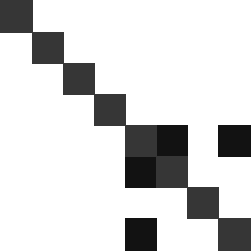
\includegraphics[width=0.31\textwidth]{figs/trap1mat} \, 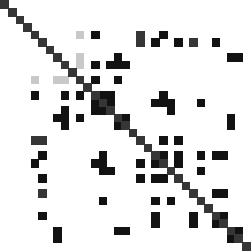
\includegraphics[width=0.31\textwidth]{figs/trap2mat} \, 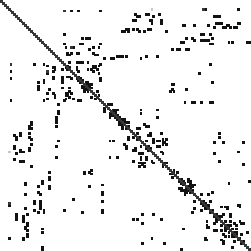
\includegraphics[width=0.31\textwidth]{figs/trap3mat}
\caption{Matrix sparsity patterns from \texttt{unfem.c} applied to the meshes \texttt{trap.1,2,3} with $N=8,33,136$ nodes, respectively.}
\label{fig:un:unfem-matsparsity}
\end{figure}

If the implementation is correct then the error will decrease at the theoretically-expected rate as the mesh is refined.  We generate nine levels of refined grids \texttt{trap.1}--\texttt{trap.9} from the following snippet of Bash code:
\begin{code}
area[0]=0.5
area[1]=0.1
area[2]=0.02
area[3]=0.005
area[4]=0.001
area[5]=0.0002
area[6]=0.00005
area[7]=0.00001
area[8]=0.000002
triangle -pqa${area[0]} meshes/trap
./tri2petsc.py meshes/trap.1 meshes/trap.1
for (( N=1; N<9; N++ )); do
    triangle -rpqa${area[$N]} meshes/trap.$N    # generate .poly,.node,.ele
    OUT=meshes/trap.$((N+1))
    ./tri2petsc.py $OUT $OUT                    # generate .vec,.is
done
\end{code}
%$

Testing of \texttt{unfem} with these meshes shows, however, that \texttt{-snes\_fd} runs are far too slow.  The runs fail with a too-many-evaluations error,\sidenote{Add \texttt{-snes\_converged\_reason} to see the error message.} for levels \texttt{trap.6}--\texttt{trap.9}.  On the other hand, the matrix-free Newton-Krylov method (Chapter \ref{chap:nl}) is also available without an assembled Jacobian.  For example, 
\begin{cline}
$ ./unfem -un_mesh meshes/trap.3 -snes_mf
case 0 result for N=136 nodes with h = 2.813e-01 :  |u-u_ex|_inf = 0.00777117
\end{cline}
%$

How far we can go with \texttt{-snes\_fd} and \texttt{-snes\_mf}?  The following snippet of Bash code uses \texttt{-snes\_mf} for those meshes for which the run completes without errors and in reasonable time:
\begin{code}
for (( N=1; N<=7; N++ )); do
    rm -f foo
    ./unfem -un_mesh meshes/trap.$N -snes_mf -log_view > foo
    grep "|u-u_ex|_inf" foo
    grep "SNESFunctionEval" foo
done
\end{code}
%$
A similar loop with ``\texttt{N=1; N<=5; N++}'' does the \texttt{-snes\_fd} runs.  The results are shown in Figure \ref{fig:un:unfem-fdmf}, which shows that errors from these runs coincide for all grids where both methods complete successfully.  These results demonstrate convergence, at a rate which we will compute using an analytical Jacobian later.

\begin{figure}
\includegraphics[width=\textwidth]{figs/unfem-fdmf}
\caption{Numerical error (open circles; left axis) and number of evaluations of \texttt{FormFunction()} (solid symbols; right axis) using \texttt{-snes\_fd} and \texttt{-snes\_mf}.}
\label{fig:un:unfem-fdmf}
\end{figure}

The runs slow-down dramatically with refinement, but the reason is no mystery.  Figure \ref{fig:un:unfem-fdmf} show the rapidly-growing number of residual evaluations as a function of the mesh spacing.  With \texttt{-snes\_fd} the number of evaluations of \texttt{FormFunction()} is proportional to the number of nodes/unknowns $N$ (Chapter \ref{chap:nl}).  By contrast, the number of residual evaluations for \texttt{-snes\_mf} scales with the number of Krylov solver iterations.  These, however, grow rapidly with refinement because, without an analytical Jacobian, or an approximation thereof, we must apply the Krylov method directly to the un-preconditioned linear system.  Option \texttt{-snes\_mf\_operator} requires the assembled matrix, addressed next.


\section{Picard iteration as a Newton-like step}

Writing additional code for an analytical Jacobian is now well-motivated.  We do not, however, construct the Jacobian in general.  Instead we build a \emph{Picard matrix}, an approximate linearization.  It is somewhat easier to construct than the Jacobian, which makes this a common technique.

To explain, observe that our nonlinear system \eqref{eq:un:fullsystem}, namely $\bF(\bu)=0$, has nearly-linear form already.\sidenote{In fact, PDE \eqref{eq:un:poissonstrong} is \emph{quasilinear} \citep{Evans2010}.}  In fact, the FEM \eqref{eq:un:weakformhat}, \eqref{eq:un:uhexpand} has the form
\begin{equation}
A(\bu) \bu = \bb(\bu) \label{eq:un:picardformsystem}
\end{equation}
for $A(\bu)\in\RR^{N\times N}$ and $\bb(\bu)\in\RR^{N}$.  Note that the residual is $\bF(\bu) = A(\bu) \bu - \bb(\bu)$.  The left side of \eqref{eq:un:weakformhat} contains all the derivative terms, which we group into the term $A(\bu) \bu$; it is regarded as a matrix-vector multiplication when computing $\bF(\bu)$.  The zeroth-order terms go into $\bb(\bu)$.  In general, and in the ``case $1$'' test problem in particular, functions $A(\bu)$ and $\bb(\bu)$ are nonlinear.

Suppose the matrix $A(\bu)$ and right-hand side $\bb(\bu)$ of \eqref{eq:un:picardformsystem} are ``frozen'' at some current iterate and the linear system solved for a new iterate:
\begin{equation}
A(\bu^k) \bu^{k+1} = \bb(\bu^k). \label{eq:un:picardnaive}
\end{equation}
This is the canonical form of \emph{Picard iteration}.\sidenote{Picard used the iteration to prove the existence of solutions to ODE IVPs (see Chapter \ref{chap:ts}) by demonstrating its convergence in that context \citep{HirschSmaleDevaney2004}.}  Under strong hypotheses on the functions $A(\bu)$ and $\bb(\bu)$, one can prove convergence of \eqref{eq:un:picardnaive}---see Exercise \ref{chap:un}.\ref{exer:un:picardconvergence}.  It is common, however, to have no more \emph{a priori} knowledge about the convergence of \eqref{eq:un:picardnaive} than we do for the Newton iteration (Chapter \ref{chap:nl}).  Similarly to \eqref{eq:un:picardnaive}, for the continuum problem \eqref{eq:un:poissonstrong} Picard iteration solves a linear PDE at each iteration:
\begin{equation}
-\Div\left(a(u^k) \grad u^{k+1}\right) = f(u^k). \label{eq:un:picardcontinuum}
\end{equation}

Our approach to \eqref{eq:un:poissonstrong} therefore \emph{could} have been to only write code---i.e.~\texttt{FormFunction()}---for the linear case with $a=a(x,y)$, $f=f(x,y)$, and then to ``hard-code'' the Picard iteration, thinking of it as \eqref{eq:un:picardnaive} or \eqref{eq:un:picardcontinuum} according to taste.  However, our actual approach is more powerful.  Instead of doing iteration \eqref{eq:un:picardnaive} as stated, we use \pSNES's line-search to globalize convergence.  Also we allow the use of the Picard matrix in pre-conditioning the Jacobian-free Newton-Krylov method---see below---so that we are actually running Newton's method using only code which assembles the Picard matrix.  These approaches become possible if we transform \eqref{eq:un:picardnaive} into Newton-like form, as follows.

Recall that the Newton method linearizes $\bF(\bu)=0$ into a system
\begin{equation}
J(\bu^k) \bs = -\bF(\bu^k),  \label{eq:un:newtonstep}
\end{equation}
for the step $\bs = \bu^{k+1}-\bu^k$.  Thus we first subtract $A(\bu^k) \bu^k$ from each side of \eqref{eq:un:picardnaive},
\begin{equation*}
A(\bu^k) (\bu^{k+1}-\bu^k) = - \left(A(\bu^k) \bu^k - \bb(\bu^k)\right).
\end{equation*}
Note the appearance of the step $\bs$, and of the residual on the right side.  We have
\begin{equation}
A(\bu^k) \bs = -\bF(\bu^k).  \label{eq:un:picardstep}
\end{equation}

Equation \eqref{eq:un:picardstep} has inserted the Picard matrix $A=A(\bu)$ where the Jacobian matrix $J=J(\bu)$ appears in \eqref{eq:un:newtonstep}.  For the linear case of PDE \eqref{eq:un:poissonstrong}, when $\partial a/\partial u=0$ and $\partial f/\partial u=0$, these matrices are the same, $A=J$.  For the general nonlinear case we expect $A$ to be a good spectral approximation of $J$ because $A$ captures the highest-order derivative terms in the PDE.  These terms  dominate the locations of the largest eigenvalues, which in turn controls the convergence of many Krylov methods (Chapter \ref{chap:ls}).


\section{Assembling and pre-allocating the Picard matrix}

Our plan is to write a function \texttt{FormPicard()} which computes a \pMat \texttt{A} $=A(\bu)$ from the current estimate $\bu$ of the solution.  Then we pass \texttt{FormPicard()} to \texttt{SNESSetJacobian()}.

Considering equations \eqref{eq:un:dirichletresiduals}, \eqref{eq:un:elementweakform}, and \eqref{eq:un:elementwisesum}, let
\begin{equation}
A_{ij}^k(\bu) = \int_{\triangle_k} a(u^h) \grad\psi_j \cdot \grad\psi_i \label{eq:un:picardentryelement}
\end{equation}
be the element-wise contribution.  The entries of $A$ are sums,
\begin{equation}
A_{ij}(\bu) =  \begin{cases}
               1, & i \in \partial_D\Omega \text{ or } j \in \partial_D\Omega, \\
               \sum_{k=0}^{K-1} A_{ij}^k(\bu), & \text{otherwise}.
               \end{cases} \label{eq:un:picardentry}
\end{equation}
This matrix is evidently symmetric and positive-definite (see \eqref{eq:un:uniformelliptic}).

We have already computed integral \eqref{eq:un:picardentryelement}, namely in evaluating \eqref{eq:un:elementintegralreference}.  Though we could re-write \texttt{FormFunction()} so that it also computes \texttt{A} as a side-effect, or we could factor out the code for the integrals \eqref{eq:un:picardentryelement} into a separate routine, it is simplest to write a separate C function \texttt{FormPicard()} because \texttt{FormFunction()}, already tested, is not touched.  In any case, for fine meshes the cost of evaluating $\bF(\bu)$ and $A(\bu)$ is small compared to the solver (below).

\texttt{FormPicard()} (not shown) is quite straightforward to write because the finicky parts of residual evaluation relate to boundary conditions---see Codes \ref{code:unfembdryresiduals} and \ref{code:unfemelementresiduals}.  One detail of note is that \texttt{MatSetValues()} is called with argument \texttt{ADD\_VALUES} to do sum \eqref{eq:un:picardentry}.

Correctly allocating memory for \pMat \texttt{A} \emph{does} matter, however.  In structured-grid cases in previous Chapters we have benefited, without being conscious of it, from \PETSc's accurate pre-allocation of memory for Jacobian matrices.  It occurs automatically when using a \pDMDA structured grid, but here we must do it ourselves.  Code \ref{code:unfemprealloc} calls \texttt{MatSeqAIJSetPreallocation()} with an array \texttt{nnz} of integers; this suffices because \texttt{unfem.c} is serial.  We compute \texttt{nnz[n]}, the number of nonzeros in row $n$ of \texttt{A}, by traversing the elements just as in \texttt{FormFunction()}.  For Dirichlet boundary nodes \texttt{nnz[n]} is one, while otherwise it is $d+1$ where $d$ is the (edge) degree of the node.  The only subtlety is that for an interior node the number of incident elements is $d-1$ while for a Neumann boundary node it is $d-2$.

Recall that Code \ref{code:unfemmain} uses \texttt{MatSetUp()} as the default alternative to calling \texttt{Preallocation()}.  For a typical matrix type, the method in \texttt{MatSetUp()} generates a dynamic list of matrix entries from calls to \texttt{MatSetValues()}.  When \texttt{MatAssemblyBegin/End()} are called it then allocates the matrix in compressed sparse row storage format (Chapter \ref{chap:ls}) and copies entries into that.  These intrinsically-expensive actions generate significant memory-system-access delays.

\cinputpart{unfem.c}{\CODELOC}{Pre-allocation of Picard matrix \pMat \texttt{A}.}{V}{//STARTPREALLOC}{//ENDPREALLOC}{code:unfemprealloc}

Pre-allocation makes a big difference.  For example, using a version of \PETSc configured with \texttt{--with-debugging=0}, we get 60 times faster performance with pre-allocation even on a medium-resolution mesh:
\begin{cline}
$ timer ./unfem -un_mesh meshes/trap.7 -un_noprealloc
case 0 result for N=46421 nodes with h = 2.210e-02 :  |u-u_ex|_inf = 6.55083e-05
real 56.30
$ timer ./unfem -un_mesh meshes/trap.7
case 0 result for N=46421 nodes with h = 2.210e-02 :  |u-u_ex|_inf = 6.55083e-05
real 0.97
\end{cline}


\section{Convergence and timing}

Now we can measure convergence down to reasonably-fine grids.  Earlier we generated grids \texttt{trap.1}--\texttt{trap.9}.  The last of these has $N\approx 10^6$ nodes and a maximum element edge length of $h=4\times 10^{-3}$.  The following Bash snippet generates the results seen in Figure \ref{fig:un:unfem-error}:
\begin{code}
for CASE in 0 1 2; do
    for N in 1 2 3 4 5 6 7 8 9; do
        ./unfem -un_mesh meshes/trap.$N -un_case $CASE -log_view
    done
done
\end{code}
Rates of convergence in the Figure are computed by logarithmic regression.
% using the results for meshes \texttt{trap.3}--\texttt{trap.8}.

\begin{figure}
\includegraphics[width=\textwidth]{figs/unfem-error}
\caption{Numerical errors and convergence rates for exact solution cases $0$, $1$, $2$, as a function of the maximum mesh edge length $h$.}
\label{fig:un:unfem-error}
\end{figure}

This evidence suggests that our code has no numerical bugs.  Though $h$ is the maximum edge length from \Triangle-generated meshes, in which we have only modest control of element shapes,\sidenote{Recall we impose an area constraint and a minimum angle condition.} the rates seen in Figure \ref{fig:un:unfem-error} are close to the theoretical rate $O(h^2)$ \citep{Braess2007}.

The runs above also used option \texttt{-log\_view}.  In \texttt{unfem.c} we added logging of stages to the code using bracketing \PETSc commands like
\begin{code}
    PetscLogStagePush(stage);
    ... action ...
    PetscLogStagePop();
\end{code}
We set stages for reading the mesh, setting-up other data structures, residual evaluation, matrix evaluation, and calling the solver (i.e.~\texttt{SNESSolve()}).  While residual and Picard matrix evaluation happen ``inside'' the solver, they are counted separately.

\begin{figure}
\includegraphics[width=\textwidth]{figs/unfem-times}
\caption{Stage times for ``case $1$'': the solver costs more than everything else.}
\label{fig:un:unfem-times}
\end{figure}

The timing results for the nonlinear ``case $1$'' runs, again using a \texttt{--with-debugging=0} version of \PETSc, is summarized in Figure \ref{fig:un:unfem-times}.  For the finer \texttt{trap.5}--\texttt{trap.9} grids\sidenote{Timing data for coarse grids is polluted by operating-system noise.} the lesson is quite clear: the solver, here ICC-preconditioned CG iteration, \emph{dominates over the cost of everything else}.  On the finest grid the solver takes about $98\%$ of the time.  Here ``everything else'' includes reading the mesh from a file, pre-allocating the \pMat, setting up \pVecs, evaluating the residual function $\bF(\bu)$, and assembling the matrix $A(\bu)$.  Note that on the finest grids there were only five evaluations of \texttt{FormFunction()} and four of \texttt{FormPicard()}.  In conclusion, our performance focus in Chapter \ref{chap:sc} will be on solvers.


\section{Preconditioned JFNK versus Picard iteration}

The above runs did Picard iteration using the matrix we assembled in \texttt{FormPicard()}.  Such an iteration is not expected to be quadratically-convergent like Newton.  We can recover quadratic convergence, however, by using the Jacobian-free Newton-Krylov (JFNK) method described in Chapter 4.  Furthermore, we can use the assembled Picard matrix from \texttt{FormPicard()} for preconditioning to reduce the number of Krylov iterations to a reasonable level.

For example, suppose we define the following common options which define a nonlinear problem (case $1$) and ask the \pSNES to fully-converge:
\begin{code}
OPTIONS="-un_mesh meshes/trap.7 -un_case 1 -snes_monitor -snes_converged_reason \
 -snes_rtol 1.0e-12 -snes_stol 1.0e-12"
\end{code}
First, Picard iteration:
\begin{cline}
$ timer ./unfem $OPTIONS
  0 SNES Function norm 3.081400684787e+01 
  1 SNES Function norm 1.870612568295e-02 
  2 SNES Function norm 4.393584241767e-05 
  3 SNES Function norm 1.499474998467e-06 
  4 SNES Function norm 3.241692297924e-07 
  5 SNES Function norm 3.808259697262e-08 
  6 SNES Function norm 4.617229888438e-09 
  7 SNES Function norm 9.102596825071e-10 
  8 SNES Function norm 9.409667934047e-11 
  9 SNES Function norm 1.413048344594e-11 
Nonlinear solve converged due to CONVERGED_FNORM_RELATIVE iterations 9
case 1 result for N=46421 nodes with h = 2.210e-02 :  |u-u_ex|_inf = 6.52846e-05
real 10.51
\end{cline}
Second is Picard-matrix-preconditioned JFNK:
\begin{cline}
$ timer ./unfem $OPTIONS -snes_mf_operator
  0 SNES Function norm 3.081400684787e+01 
  1 SNES Function norm 2.103388830244e+01 
  2 SNES Function norm 3.074978769509e+00 
  3 SNES Function norm 1.272280930525e-01 
  4 SNES Function norm 3.523741442353e-04 
  5 SNES Function norm 3.959655045717e-09 
  6 SNES Function norm 8.861144493199e-14 
Nonlinear solve converged due to CONVERGED_FNORM_RELATIVE iterations 6
case 1 result for N=46421 nodes with h = 2.210e-02 :  |u-u_ex|_inf = 6.52847e-05
real 33.85
\end{cline}
A third run with \texttt{-snes\_mf}, i.e.~un-preconditioned JFNK, shows the same number of iterations, and nearly the same residual norms, but takes $77$ seconds.

This is interesting.  The Picard-iteration run is distinctly faster.  Also it shows a big drop in residual in the first few iterations, but then the residual norm decreases by roughly an order-of-magnitude per iteration.  By contrast, the second and third runs show quadratic convergence with a classic drop in the residual norm.

In summary, the Picard matrix can indeed be used to precondition the linear system arising from finite-difference approximation of the the action of the Jacobian (i.e.~\texttt{-snes\_mf\_operator} as JFNK).  However, the Picard step itself is a surprisingly good one in this case, despite not being the exact linearization around the current iterate.  The timing difference above is certainly related to the number of Krylov iterations taken, requiring more work to diagnose.\sidenote{Start by adding \texttt{-ksp\_converged\_reason} and \texttt{-snes\_view}.}

It is not clear how general this situation is.  Nor is there a ``conclusion'' to offer.  We can, however, say confidently that if the user writes code to assemble a Picard-type linearization then both Picard iteration and Picard-preconditioned JFNK are available options at the \PETSc command line.


\section{Performance relative to \pDMDA structured grid}

It is a reasonable question to ask whether a given code is ``efficient.''  For \texttt{unfem.c} there is even a reasonable \emph{answer}.  This assumes that \PETSc \pDMDA handles structured-grid problems efficiently.  We will run \texttt{unfem.c} on a structured grid---managed as though it is an unstructured triangulation---and then compare timing and numerical error from a code using a \pDMDA for the same grid.

First we generate a triangulation, in \Triangle format, for the unit square domain $\mathcal{S}=(0,1)\times (0,1)$ using Python script \texttt{c/ch7/genstructured.py} (not shown).  For example the commands
\begin{cline}
$ ./genstructured.py foursquare 4
...
$ showme foursquare
\end{cline}
%$
generate and then view the small grid shown in Figure \ref{fig:un:smallstructured}.

\begin{marginfigure}
\input{tmp/mesh.1.tikz}
\caption{A structured triangulation on the unit square with $N=16$ nodes.}
\label{fig:un:smallstructured}
\end{marginfigure}

An additional ``case $3$'' is implemented in \texttt{unfem.c} for this square domain.  This linear problem, with exclusively Dirichlet boundary conditions and an exact solution, is the one also solved by \texttt{poisson.c} in Chapter \ref{chap:st}.  We run this case, for a \texttt{--with-debugging=0} build, on a fine grid with $2^{10}=1024$ subintervals in each direction, and thus $N=1025^2$ unknowns:
\begin{cline}
$ ./genstructured.py square 1025
...
$ ./tri2petsc.py square square
...
$ timer ./unfem -un_mesh square -un_case 3
case 3 result for N=1050625 nodes with h = 1.381e-03 :  |u-u_ex|_inf = 9.89813e-08
real 24.47
\end{cline}
%$
Compare the result from \texttt{poisson.c}, which uses \pDMDA and finite differences:
\begin{cline}
$ cd ../ch3/
$ make poisson
...
$ timer ./poisson -da_refine 7 -ksp_type cg -pc_type icc
on 1025 x 1025 grid:  error |u-uexact|_inf = 5.29691e-08
real 18.67
\end{cline}
%$
The timing and error are very similar.

The message is clear.  Our approach, which consists especially of
\begin{itemize}
\item reading an unstructured mesh from \PETSc binary files,
\item evaluating the residual and Picard matrix by traversing the boundary and elements using unstructured indexing,
\item using \pSNES even on a linear problem, and
\item pre-allocating the matrix by traversal of the elements
\end{itemize}
is nearly as fast as using finite differences on a \pDMDA structured grid.


\section{Poisson equation on the Koch snowflake}

As convergence and timing results become sterile after a while, here is a diversion just for fun.

The polygonal domain on the left in Figure \ref{fig:un:kochpolygonmesh} is an early stage in a construction of the \emph{Koch snowflake}, one of the first fractals \citep{vonKoch1904}.  An unstructured mesh is natural for solving a PDE on such a complicated polygonal domain.  In the case shown the polygon was generated by a Python script \texttt{polygon.py} in \texttt{c/ch7/koch/} (not shown), and the triangulation was generated by \Triangle:
\begin{cline}
$ cd c/ch7/koch/
$ ./polygon.py -l 2 -o koch.poly
$ triangle -pqa0.025 koch.poly
\end{cline}
%$
The polygon is second-level (\texttt{-l 2}) while the fractal would be the $\infty$-level.

\begin{figure}
\input{tmp/koch.tikz} \qquad \input{tmp/koch.1.tikz}
\caption{An early stage in the construction of the Koch snowflake (left) and a triangulation thereof (right).}
\label{fig:un:kochpolygonmesh}
\end{figure}

Code \texttt{unfem} can solve a Poisson equation on any level of Koch polygonal domain $\Omega$.  Consider the simple example of homogeneous Dirichlet boundary conditions and $a(u)=f(u)=1$ in form \eqref{eq:un:poissonstrong},
\begin{equation}
-\grad^2 u = 1.\label{eq:un:kochpoisson}
\end{equation}
A ``case $4$'' has been added to \texttt{c/ch7/cases.h} for this problem.  It is a model, for example, of the steady state of a diffusion process on $\Omega$ with constant production in the interior and absorption on the boundary.

The following computes a level-five polygon with $P\approx 3\times 10^3$ segments and generates a \PETSc-binary-format mesh with $N\approx 8\times 10^4$ nodes:
\begin{cline}
$ ./polygon.py -l 5 -o koch5.poly
$ triangle -pqa0.00002 koch5.poly
$ ../tri2petsc.py koch5.1 koch5.1
\end{cline}
%$
Then we solve the above Poisson equation:
\begin{cline}
$ ../unfem -un_mesh koch5.1 -un_case 4 -un_view_solution \
    -snes_monitor -ksp_converged_reason
\end{cline}
%$
(Option \texttt{-un\_view\_solution} saves a \PETSc-binary-format file \texttt{koch5.1.soln} containing the solution $u$ at each node.)  Application of Python script \texttt{c/ch7/petsc2tricontour.py}, with specific contours to show details near the boundary, generates Figure \ref{fig:un:snowflake}:
\begin{cline}
$ export CONTOURS="1e-6 1e-5 3e-5 1e-4 3e-4 0.001 0.003 0.01 0.02 0.03 0.05 0.1"
$ ../petsc2contour.py -i koch5.1 --contours $CONTOURS
\end{cline}
%$

\begin{figure}
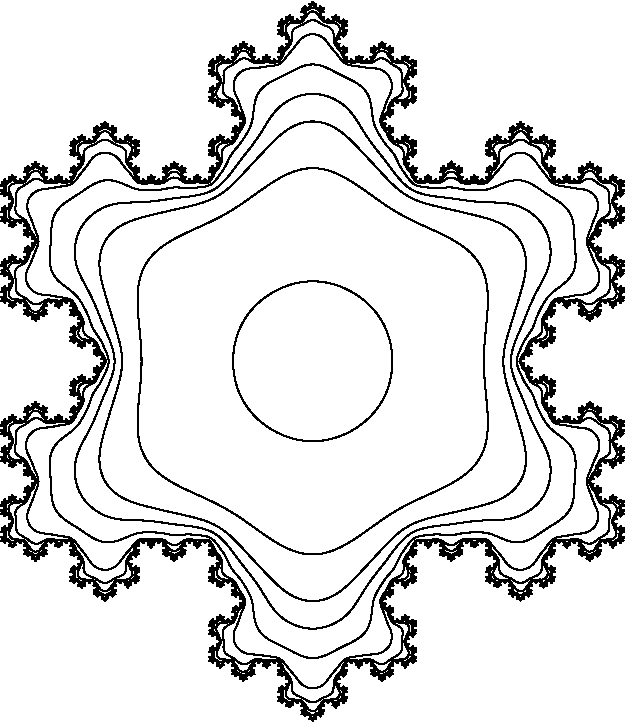
\includegraphics[width=0.8\textwidth]{figs/snowflake}
\caption{Solution of Poisson problem \eqref{eq:un:kochpoisson} on an approximation of the Koch snowflake fractal.}
\label{fig:un:snowflake}
\end{figure}


\section{Toward parallel unstructured meshes}

This Chapter's relatively-naive approach to unstructured meshes is acceptable for serial computations, but it must be completely transformed in parallel.  In Chapter \ref{chap:dp} we will use \PETSc tools for parallel unstructured meshes, but a strategy based on the tools in the current Chapter can be sketched.

Generating the mesh itself in parallel is outside of our scope.  Thus we assume that the mesh is already given in a file, however generated, with nodes and elements\sidenote{And the boundary nodes and segments, but we ignore the boundary in this sketch.} numbered by the same indexing scheme as in this Chapter.  This is the ``global'' indexing.

Because we integrate the weak form \eqref{eq:un:poissonweak} element-by-element, in parallel each element is owned by exactly one process.  Thus the list of \emph{elements} is partitioned across the processors (Figure \ref{fig:un:parallelunstructured}).  Such a disjoint element partitioning induces a list of nodes, and FEM unknowns, which must be accessible on a given process.  The same basic facts apply to edges, although boundary segments do have an (induced) disjoint partition.  Shared nodes may be regarded as ``ghost'' nodes on neighboring processors (Figure \ref{fig:petscghostvalues}).

\begin{figure}

\begin{tikzpicture}[scale=0.7]
% rank 0 elements
\pgfmathsetmacro{\xo}{0.0}
\pgfmathsetmacro{\yo}{0.0}

  \filldraw[fill=gray!50, draw=black] (0.000000+\xo,-2.000000+\yo) -- (1.828947+\xo,-0.947368+\yo) -- (0.000000+\xo,0.000000+\yo) -- (0.000000+\xo,-2.000000+\yo) ;
  \filldraw[fill=gray!50, draw=black] (2.000000+\xo,-3.000000+\yo) -- (1.828947+\xo,-0.947368+\yo) -- (0.000000+\xo,-2.000000+\yo) -- (2.000000+\xo,-3.000000+\yo) ;
  \filldraw[fill=gray!50, draw=black] (0.000000+\xo,0.000000+\yo) -- (1.828947+\xo,-0.947368+\yo) -- (2.500000+\xo,1.000000+\yo) -- (0.000000+\xo,0.000000+\yo) ;
  \filldraw[fill=gray!50, draw=black] (1.828947+\xo,-0.947368+\yo) -- (2.000000+\xo,-3.000000+\yo) -- (4.000000+\xo,-1.799890+\yo) -- (1.828947+\xo,-0.947368+\yo) ;
  \draw[black] (4.000000+\xo,-1.799890+\yo) -- (5.957182+\xo,-0.804788+\yo) -- (2.500000+\xo,1.000000+\yo) -- (4.000000+\xo,-1.799890+\yo) ;
  \draw[black] (2.500000+\xo,1.000000+\yo) -- (1.828947+\xo,-0.947368+\yo) -- (4.000000+\xo,-1.799890+\yo) -- (2.500000+\xo,1.000000+\yo) ;
  \draw[black] (2.500000+\xo,1.000000+\yo) -- (5.957182+\xo,-0.804788+\yo) -- (5.000000+\xo,2.000000+\yo) -- (2.500000+\xo,1.000000+\yo) ;

% rank 1 elements
\pgfmathsetmacro{\xo}{8.0}
\pgfmathsetmacro{\yo}{0.0}

  \draw[black] (0.000000+\xo,-2.000000+\yo) -- (1.828947+\xo,-0.947368+\yo) -- (0.000000+\xo,0.000000+\yo) -- (0.000000+\xo,-2.000000+\yo) ;
  \draw[black] (2.000000+\xo,-3.000000+\yo) -- (1.828947+\xo,-0.947368+\yo) -- (0.000000+\xo,-2.000000+\yo) -- (2.000000+\xo,-3.000000+\yo) ;
  \draw[black] (0.000000+\xo,0.000000+\yo) -- (1.828947+\xo,-0.947368+\yo) -- (2.500000+\xo,1.000000+\yo) -- (0.000000+\xo,0.000000+\yo) ;
  \draw[black] (1.828947+\xo,-0.947368+\yo) -- (2.000000+\xo,-3.000000+\yo) -- (4.000000+\xo,-1.799890+\yo) -- (1.828947+\xo,-0.947368+\yo) ;
  \filldraw[fill=gray!50, draw=black] (4.000000+\xo,-1.799890+\yo) -- (5.957182+\xo,-0.804788+\yo) -- (2.500000+\xo,1.000000+\yo) -- (4.000000+\xo,-1.799890+\yo) ;
  \filldraw[fill=gray!50, draw=black] (2.500000+\xo,1.000000+\yo) -- (1.828947+\xo,-0.947368+\yo) -- (4.000000+\xo,-1.799890+\yo) -- (2.500000+\xo,1.000000+\yo) ;
  \filldraw[fill=gray!50, draw=black] (2.500000+\xo,1.000000+\yo) -- (5.957182+\xo,-0.804788+\yo) -- (5.000000+\xo,2.000000+\yo) -- (2.500000+\xo,1.000000+\yo) ;

% labels
  \node at (2.8,-4.2) {rank $0$};
  \node at (2.8+\xo,-4.2) {rank $1$};

% rank 0 nodes
\pgfmathsetmacro{\xo}{0.0}
\pgfmathsetmacro{\yo}{-7.0}
\newcommand{\ldot}{node[circle,fill=black,inner sep=1.0pt] (0.0pt) {.}}
\newcommand{\rdot}{}
\newcommand{\gdot}{node[circle,draw,gray,thick,inner sep=3.0pt] (0.0pt) {.}}

  \draw[black] (0.000000+\xo,-2.000000+\yo) \ldot -- (1.828947+\xo,-0.947368+\yo) \ldot -- (0.000000+\xo,0.000000+\yo) \ldot -- (0.000000+\xo,-2.000000+\yo) ;
  \draw[black] (2.000000+\xo,-3.000000+\yo) \ldot -- (1.828947+\xo,-0.947368+\yo) \ldot -- (0.000000+\xo,-2.000000+\yo) \ldot -- (2.000000+\xo,-3.000000+\yo) ;
  \draw[black] (0.000000+\xo,0.000000+\yo) \ldot -- (1.828947+\xo,-0.947368+\yo) \ldot -- (2.500000+\xo,1.000000+\yo) \ldot -- (0.000000+\xo,0.000000+\yo) ;
  \draw[black] (1.828947+\xo,-0.947368+\yo) \ldot -- (2.000000+\xo,-3.000000+\yo) \ldot -- (4.000000+\xo,-1.799890+\yo) \ldot -- (1.828947+\xo,-0.947368+\yo) ;
  \draw[black] (4.000000+\xo,-1.799890+\yo) \rdot -- (5.957182+\xo,-0.804788+\yo) \rdot -- (2.500000+\xo,1.000000+\yo) \rdot -- (4.000000+\xo,-1.799890+\yo) ;
  \draw[black] (2.500000+\xo,1.000000+\yo) \rdot -- (1.828947+\xo,-0.947368+\yo) \rdot -- (4.000000+\xo,-1.799890+\yo) \rdot -- (2.500000+\xo,1.000000+\yo) ;
  \draw[black] (2.500000+\xo,1.000000+\yo) \rdot -- (5.957182+\xo,-0.804788+\yo) \rdot -- (5.000000+\xo,2.000000+\yo) \rdot -- (2.500000+\xo,1.000000+\yo) ;
  % shared nodes:
  \draw[black] (2.500000+\xo,1.000000+\yo) \gdot -- (1.828947+\xo,-0.947368+\yo) \gdot -- (4.000000+\xo,-1.799890+\yo) \gdot -- (2.500000+\xo,1.000000+\yo) ;

% rank 1 nodes
\pgfmathsetmacro{\xo}{8.0}
\pgfmathsetmacro{\yo}{-7.0}
\renewcommand{\ldot}{}
\renewcommand{\rdot}{node[circle,fill=black,inner sep=1.0pt] (0.0pt) {.}}

  \draw[black] (0.000000+\xo,-2.000000+\yo) \ldot -- (1.828947+\xo,-0.947368+\yo) \ldot -- (0.000000+\xo,0.000000+\yo) \ldot -- (0.000000+\xo,-2.000000+\yo) ;
  \draw[black] (2.000000+\xo,-3.000000+\yo) \ldot -- (1.828947+\xo,-0.947368+\yo) \ldot -- (0.000000+\xo,-2.000000+\yo) \ldot -- (2.000000+\xo,-3.000000+\yo) ;
  \draw[black] (0.000000+\xo,0.000000+\yo) \ldot -- (1.828947+\xo,-0.947368+\yo) \ldot -- (2.500000+\xo,1.000000+\yo) \ldot -- (0.000000+\xo,0.000000+\yo) ;
  \draw[black] (1.828947+\xo,-0.947368+\yo) \ldot -- (2.000000+\xo,-3.000000+\yo) \ldot -- (4.000000+\xo,-1.799890+\yo) \ldot -- (1.828947+\xo,-0.947368+\yo) ;
  \draw[black] (4.000000+\xo,-1.799890+\yo) \rdot -- (5.957182+\xo,-0.804788+\yo) \rdot -- (2.500000+\xo,1.000000+\yo) \rdot -- (4.000000+\xo,-1.799890+\yo) ;
  \draw[black] (2.500000+\xo,1.000000+\yo) \rdot -- (1.828947+\xo,-0.947368+\yo) \rdot -- (4.000000+\xo,-1.799890+\yo) \rdot -- (2.500000+\xo,1.000000+\yo) ;
  \draw[black] (2.500000+\xo,1.000000+\yo) \rdot -- (5.957182+\xo,-0.804788+\yo) \rdot -- (5.000000+\xo,2.000000+\yo) \rdot -- (2.500000+\xo,1.000000+\yo) ;
  % shared nodes:
  \draw[black] (2.500000+\xo,1.000000+\yo) \gdot -- (1.828947+\xo,-0.947368+\yo) \gdot -- (4.000000+\xo,-1.799890+\yo) \gdot -- (2.500000+\xo,1.000000+\yo) ;
  
\end{tikzpicture}


\caption{In a parallel partition of an unstructured mesh, elements (top) are uniquely-owned by processes, but nodes (bottom) may be shared (gray circles).}
\label{fig:un:parallelunstructured}
\end{figure}

Partitioning is not done by \PETSc either, but it can be done in parallel by using ParMETIS \citep{KarypisKumar1999}, for example.  The partitioning could seek geometrically-compact partitions, or it could be based on load-balancing considerations.  The goal of ParMETIS is to reduce inter-process communication by seeking to minimize the number of edges which are incident to elements in different partitions, while balancing the number of elements.

The element partitioning can be recorded in a \texttt{MatPartitioning} object and an integer-entry adjacency matrix of type \texttt{MATMPIADJ}.\sidenote{For the naive approach in the current Chapter, \Triangle's \texttt{.neigh} file provides the adjacency graph for the elements.}  Each process calls \texttt{MatCreateMPIAdj()} with, in essense, a list of which elements it owns.  One may then generate additional indexing structures so that each processor can use to get ``local'' indexing for its patch \citep{petsc-user-ref}.  Then each process loops over its elements computing the element contributions to integrals using the local numbering of the vertices.

Implementing the above strategy as naively as in this Chapter would be possible, but it is unnecessary because \PETSc contains tools for these jobs.  The above steps can be treated more abstractly.  Note that the highest-dimensional geometric objects in the triangulation are the elements.  If they are disjointly-partitioned then the operation needed in doing element-by-element assembly of the residual (or stiffness matrix, etc.) requires the ``closure'' of lower-dimensional objects (i.e.~edges and nodes) incident to a given element.  In fact one would want a \pVec with the values of the unknown function $u(x,y)$, for example, at all nodes in the closure of the owned elements, for example.  These concepts are demonstrated, based on applying the \pDMPlex type, in Chapter \ref{chap:dp}.


\section{Exercises}

\renewcommand{\labelenumi}{\arabic{chapter}.\arabic{enumi}\quad}
\renewcommand{\labelenumii}{(\alph{enumii})}
\begin{enumerate}
\item \label{exer:un:notminimization}  The text asserts that our PDE problem \eqref{eq:un:poissonstrong} does not generally arise from a minimization principle.  This Exercise expands on the claim.  For simplicity suppose that $f$ is independent of $u$, use homogeneous Dirichlet boundary conditions on $\partial \Omega$.  (Also, feel free to consider only the 1D version of the problem.)  First show, by following the technique that derived \eqref{eq:of:plapweakform}, that if $\partial a/\partial u \ne 0$ then the Euler-Lagrange equation of
\begin{equation}
  \tilde I[u] = \int_\Omega \frac{1}{2} a(u) |\grad u|^2 - f u,  \label{eq:un:nottheobjective}
\end{equation}
a reasonable guess, is \emph{not} the weak form \eqref{eq:un:poissonweak}.  This does not exclude that some other minimization problem leads to \eqref{eq:un:poissonweak}, however.  Therefore, show next that if $\partial a/\partial u \ne 0$ then the residuals \eqref{eq:un:elementwisesum} satisfy
\begin{equation}
  \frac{\partial F_i(u)}{\partial u_j} \ne \frac{\partial F_j(u)}{\partial u_i} \label{eq:un:symmetryresidualsdonthave}
\end{equation}
for some $u$.  Explain why this \emph{does} exclude minimization.
\item  \label{exer:un:gradientdetails}  For the map \eqref{eq:un:trianglemap} from $\triangle_\ast$ to $\triangle_k$, note
    $$J_k = \frac{\partial (x,y)}{\partial (\xi,\eta)} = \begin{pmatrix}
    x_1 - x_0 & x_2 - x_0 \\
    y_1 - y_0 & y_2 - y_0 \end{pmatrix}
    = \begin{pmatrix}
    \Delta x_1 & \Delta x_2 \\
    \Delta y_1 & \Delta y_2
    \end{pmatrix}$$
is the Jacobian.  Use the chain rule and \eqref{eq:un:psichimap} to show that
\begin{equation}
\grad_{x,y} \psi_i = \frac{1}{\det J_k} \left<\Delta y_2 \frac{\partial \chi_\ell}{\partial \xi} - \Delta y_1 \frac{\partial \chi_\ell}{\partial \eta}, - \Delta x_2 \frac{\partial \chi_\ell}{\partial \xi} + \Delta x_1 \frac{\partial \chi_\ell}{\partial \eta}\right>. \label{eq:un:gradpsionref}
\end{equation}
Here indices $i$ and $\ell$ have the same relationship as in \eqref{eq:un:psichimap}.  Compare formula \eqref{eq:of:gradpsionref} for the structured case.
\item  \label{exer:un:elementintegranddetails}  Formula \eqref{eq:un:elementintegrand} might require some interpretation before the implementation becomes clear, and thus this Exercise.  Confirm that formulas \eqref{eq:un:trianglemap} and \eqref{eq:un:psichimap} lead to the following expansions of expressions, which together make \eqref{eq:un:elementintegrand} implementable:
\begin{align}
a(u^h) &= a(u^h,x(\xi,\eta),y(\xi,\eta)), \label{eq:un:adetails} \\
f(u^h) &= f(u^h,x(\xi,\eta),y(\xi,\eta)), \label{eq:un:fdetails} \\
\psi_i &= \chi_{\ell}(\xi,\eta), \label{eq:un:psichidetails} \\
u^h &= \sum_{j=0}^{N-1} \left\{\begin{matrix} g_D(\bx_j) \\ u_j \end{matrix}\right\} \chi_{\ell'}(\xi,\eta), \label{eq:un:udetails} \\
\grad u^h &= \grad_{x,y} u^h = \sum_{j=0}^{N-1} \left\{\begin{matrix} g_D(\bx_j) \\ u_j \end{matrix}\right\} \grad_{x,y} \psi_j. \label{eq:un:gradudetails}
\end{align}
In \eqref{eq:un:psichidetails} the node $\bx_i$ corresponds to vertex $\ell$ on $\triangle_\ast$.  In \eqref{eq:un:udetails} and \eqref{eq:un:gradudetails}, the two cases for computing the coefficient are when $\bx_j \in \partial_D \Omega$ and $\bx_j \notin \partial_D \Omega$, respectively; also note that node $\bx_j$ corresponds to vertex $\ell'$ on $\triangle_\ast$.  Note that \eqref{eq:un:gradpsionref} allows us to expand $\grad_{x,y} \psi_j$ in \eqref{eq:un:gradudetails}.
\item  \label{exer:un:checkquadrature}  The degree of accuracy $n=1,2,3$ of the quadrature rules in Table \ref{tab:un:quadrature} can be checked by comparing the exact integral
\begin{equation}
\iint_{\triangle_\ast} \xi^i \eta^j\,d\xi d\eta = \frac{i!\,j!}{(i+j+2)!}, \label{eq:un:checkquadrature}
\end{equation}
for all cases with $0\le i+j\le n$, against the quadrature result.  Also one can show that the quadrature result is \emph{not} exact for some case with $i+j=n+1$.  Write a small program, in the language of your choice, which checks these assertions.
\item \label{exer:un:gaussneumann}  In \texttt{unfem.c} we use the midpoint rule when computing the Neumann boundary segment contributions $\varphi_\nu^i$; see equation \eqref{eq:un:segmentquadrature}.  Modify \texttt{unfem.c} to optionally use two-point Gaussian quadrature instead.  Only in case 2 will this make any difference.  Show that accuracy noticeably improves for coarse grids, but that this benefit disappears under grid refinement.
% see c/ch7/solns/segmentgauss.c.snippet
\item \label{exer:un:picardconvergence}  In this Exercise about Picard iteration let $\|\cdot\|$ denote the $2$-norm: $\|w\| = \sqrt{\bw^\top \bw}$ for $\bw\in\RR^N$.  Assume that the right-hand side of \eqref{eq:un:picardnaive} is bounded, $\|\bb(\bu)\| \le B_b$, and that the functions are Lipschitz, $\|A(\bu)-A(\bv)\| \le L_A \|\bu-\bv\|$ and $\|\bb(\bu)-\bb(\bv)\| \le L_b \|\bu-\bv\|$.  Assume also that $A(\bu)$ is uniformly positive-definite, so that there is $\delta>0$ for which $\bw^\top A(\bu) \bw \ge \|\bw\|^2/\delta$ for all $\bu, \bw \in \RR^N$; equivalently this says $\|A^{-1}(\bu)\| \le \delta$.  (\emph{For the FEM matrix in this Chapter, the existence of $\delta$ follows from uniform-ellipticity assumption \eqref{eq:un:uniformelliptic}.})  Show that the sequence generated by \eqref{eq:un:picardnaive} is well-defined and bounded, $\|\bu_k\| \le \delta B_b$.  Now let $\alpha = \delta \left(L_A B_b \delta + L_b\right)$.  Show that \eqref{eq:un:picardnaive} satisfies $\|\bu^{k+1}-\bu^{k}\| \le \alpha \|\bu^{k}-\bu^{k-1}\|$ under the (very strong) assumption that $\alpha < 1$.  It follows from a geometric series argument that the Picard iteration converges; show this.  (\emph{These norm techniques for analysing Picard iteration are more useful when applied to ODE IVPs \citep{HirschSmaleDevaney2004}.  In that case the map is close to the identity for small time intervals $[0,T]$, and the analog of ``$\alpha$'' scales with $T$ and the relevant Lipschitz constant.  Thus existence is easy to show for small times.})
\item Explain why the first of these two runs, which each solve the (default) linear ``case $0$'' problem, requires fewer \pSNES iterations:
\begin{cline}
$ ./unfem -un_mesh meshes/trap.3 -snes_monitor -ksp_rtol 1.0e-14
$ ./unfem -un_mesh meshes/trap.3 -snes_monitor -ksp_rtol 1.0e-14 -snes_fd
\end{cline}
Now explain why the \emph{second} of these two runs, which solve the nonlinear ``case $1$'' problem, requires fewer \pSNES iterations:
\begin{cline}
$ ./unfem -un_case 1 -un_mesh meshes/trap.3 -snes_monitor
$ ./unfem -un_case 1 -un_mesh meshes/trap.3 -snes_monitor -snes_fd
\end{cline}
(\emph{If it is clear then congratulations!  You are becoming a \pSNES pro.})
\item The result of
\begin{cline}
$ ./unfem -un_mesh meshes/trapneu.1 -un_case 2
\end{cline}
%$
is a numerical error of zero; why?  (\emph{This explains a missing marker on the coarsest grid in Figure \ref{fig:un:unfem-error}.})
\item The default quadrature degree corresponds to option \texttt{-un\_quaddeg 1}.  To try all the implemented degrees do something like this:
\begin{code}
for CASE in 0 1; do
    for DEG in 1 2 3; do
        ./unfem -un_mesh meshes/trap.3 -un_case $CASE -un_quaddeg $DEG -snes_converged_reason
    done
done
\end{code}
Why is the difference between degrees $1$ and $2$ only substantial in the nonlinear ``case $1$''?  Why isn't there a larger difference between degrees $2$ and $3$?
\item \label{exer:un:allneumannfailure}  We have assumed that the Dirichlet boundary $\partial_D \Omega$ has positive measure (length) so that the linear problem, at least, is known to have a unique solution.  By contrast, confirm experimentally that if $\partial_D\Omega$ is empty then the equations no longer have a unique solution.  This can be done by modifying the ``case $2$'' exact solution to use only Neumann boundary conditions.  A direct solve for the linear equations (\texttt{-ksp\_type preonly -pc\_type lu}) will fail; explain the error message which results.
\item \label{exer:un:allneumannresolution}  FIXME Continuing the above Exercise, use \texttt{SNESGetKSP()} and \texttt{KSPSetNullSpace()} to tell the linear solver that the linearization of the Neumann-only problem has constant functions as its null space.  Confirm that direct and iterative solvers now succeed as in the case with non-empty Dirichlet boundary.
\item \label{exer:un:truejacobian} Implement the true Jacobian in the $a=a(x,y)$ case, that is, with the correct linearization when $\partial f/\partial u\ne 0$.  This will add a diagonal term to the matrix.  A test case is appropriate, and, in preparation for the next Exercise, it might be built by manufacturing a solution to the equation $-\nabla^2 u = f(u,x,y)$ where $f(u,x,y) = e^u + F(x,y)$ and where $F(x,y)$ is generated by differentiation from a chosen exact solution.  Compare results from Picard and Newton iteration in this case.  (\emph{This exercise requires a bit of coding.  In preparation for the next problem you may want to call your new code \texttt{bratu2.c}, starting it from a copy of \texttt{unfem.c}, with appropriately modified makefile.})
\item \label{exer:un:bratu} Use the code from the previous Exercise to solve the Bratu equation $-\nabla^2 u = \lambda e^u$ with homogeneous Dirichlet boundary conditions on the unit square $\mathcal{S}=(0,1)\times(0,1)$.  Compute the critical value of $\lambda$ as you did in the 1D problem in Exercise \ref{eq:nl:bratuoned}, again comparing results from Picard and Newton iteration.
% equals 6.81 according to \pSNES example \texttt{ex5.c}
\item \label{exer:un:robin} Implement and test a version of \texttt{unfem.c} which can handle Robin boundary conditions.
\end{enumerate}

